\documentclass[11pt]{article}

% arXiv-compatible preamble
\usepackage[utf8]{inputenc}
\usepackage[T1]{fontenc}
\usepackage{lmodern}
\usepackage{graphicx}
\usepackage{amsmath}
\usepackage{amssymb}
\usepackage{cite}
\usepackage{hyperref}
\usepackage[margin=1in]{geometry}
\usepackage{setspace}
\usepackage{fancyhdr}
\usepackage{float}
\usepackage{booktabs}
\usepackage{array}
\usepackage{xcolor}

% Set spacing
\setstretch{1.15}

% Define graphicspath for figures in plots/ subdirectory
\graphicspath{{./plots/}{plots/}{./}{.}}

% Metadata
\title{Awesome Awesomers: Mapping Influence \& Impact in Tech Communities\\
{\large A Two-Phase Comparative Analysis of Influential Technologists and Awesome-Repository Curators}}

\author{
    Pelayo González de Lena Rodríguez$^{1,2,\dagger}$
}

\date{March 17, 2026}

% Affiliations
\newcommand{\affiliations}{%
    $^{1}$Department of Organisms and Systems Biology (BOS), ValMeiLab, Faculty of Biology, University of Oviedo, Oviedo, Spain\\
    $^{2}$Cancer Epigenomics and Nanomedicine Laboratory (EpiLab), ISPA-FINBA / CINN-CSIC, Oviedo, Spain\\
    $^{\dagger}$Corresponding author: \texttt{pelayo.gonzalez@uniovi.es}
}

\begin{document}

% Title page
\maketitle

\vspace{0.5cm}
\begin{center}
\small
\affiliations
\end{center}

\vspace{1cm}

% Abstract
\begin{abstract}
This paper presents a two-phase comparative analysis of influence and impact in technology communities. Phase 1 analyzes 74 influential technologists across AI/ML, bioinformatics, and data science domains, identifying power-law distribution patterns in follower counts (Zipf exponent $\alpha = 0.62$) with strong positive correlation between followers and total stars ($\rho = 0.58$, $p < 0.001$). Phase 2 examines 21 curators of awesome-* repositories (179 repos, 4.2M total stars), revealing distinct success pathways ($\rho = 0.31$, independent metrics). Network analysis identifies 5 communities in Phase 1 and 4 in Phase 2, with betweenness centrality revealing key knowledge brokers. Results demonstrate that influence in tech is driven by different incentive structures: Phase 1 emphasizes brand-building through follower accumulation, while Phase 2 prioritizes niche expertise and curation quality. The study provides quantitative evidence for understanding community dynamics and knowledge dissemination in open-source and technology sectors.

\vspace{0.5cm}
\noindent
\textbf{Keywords:} influence networks, open-source communities, GitHub, curators, power-law distributions, network analysis, knowledge brokers

\end{abstract}

\newpage
\tableofcontents
\newpage

% ============================================================================
% 1. INTRODUCTION
% ============================================================================

\section{Introduction}

The technology landscape has undergone a fundamental transformation in the past two decades, with the rise of open-source software, GitHub-based collaboration, and influential technologists shaping the trajectory of fields from artificial intelligence to bioinformatics. Understanding the mechanisms of influence in these communities is essential for both researchers and practitioners seeking to identify thought leaders and understand how knowledge disseminates.

Previous work has examined influence in social networks \cite{newman2018networks}, power-law distributions in online communities \cite{barabasi2009scale}, and the role of hubs in knowledge networks \cite{watts1998collective}. However, few studies have directly compared two distinct classes of influential actors: individual technologists (who build personal brands through Twitter/GitHub presence) and curators (who aggregate and organize community knowledge through awesome-* repositories).

This study addresses three research questions:

\begin{enumerate}
    \item How does influence manifest differently in individual technologists versus repository curators?
    \item Do follower counts, repository metrics, and engagement measures follow power-law distributions?
    \item What network structures emerge when we examine communities of practice within these two populations?
\end{enumerate}

\section{Related Work}

\subsection{Influence and Network Analysis}

The concept of influence in social networks has been extensively studied. Kwak et al. \cite{kwak2010} analyzed Twitter as a social network, demonstrating that follower counts exhibit power-law distributions. Granovetter \cite{granovetter1973} introduced the concept of ``weak ties'' as critical connectors in networks, a finding that has profound implications for understanding influence and information flow.

\subsection{Open Source Communities}

Open-source software development has become central to modern technology. Crowston and Howison \cite{crowston2006} examined the evolution and sustainability of open-source projects. More recently, Eghbal \cite{eghbal2016} highlighted the critical role of maintainers and curators in sustaining open-source ecosystems.

\subsection{Awesome Lists as Knowledge Infrastructure}

The awesome-* repository ecosystem emerged organically from Sindre Sorhus's original \texttt{awesome} list in 2013. These repositories serve as meta-repositories of curated resources, representing a form of distributed knowledge organization. To our knowledge, this is the first quantitative analysis of the awesome-* ecosystem as a whole.

% ============================================================================
% 2. METHODS
% ============================================================================

\section{Methods}

\begin{figure}[H]
\centering
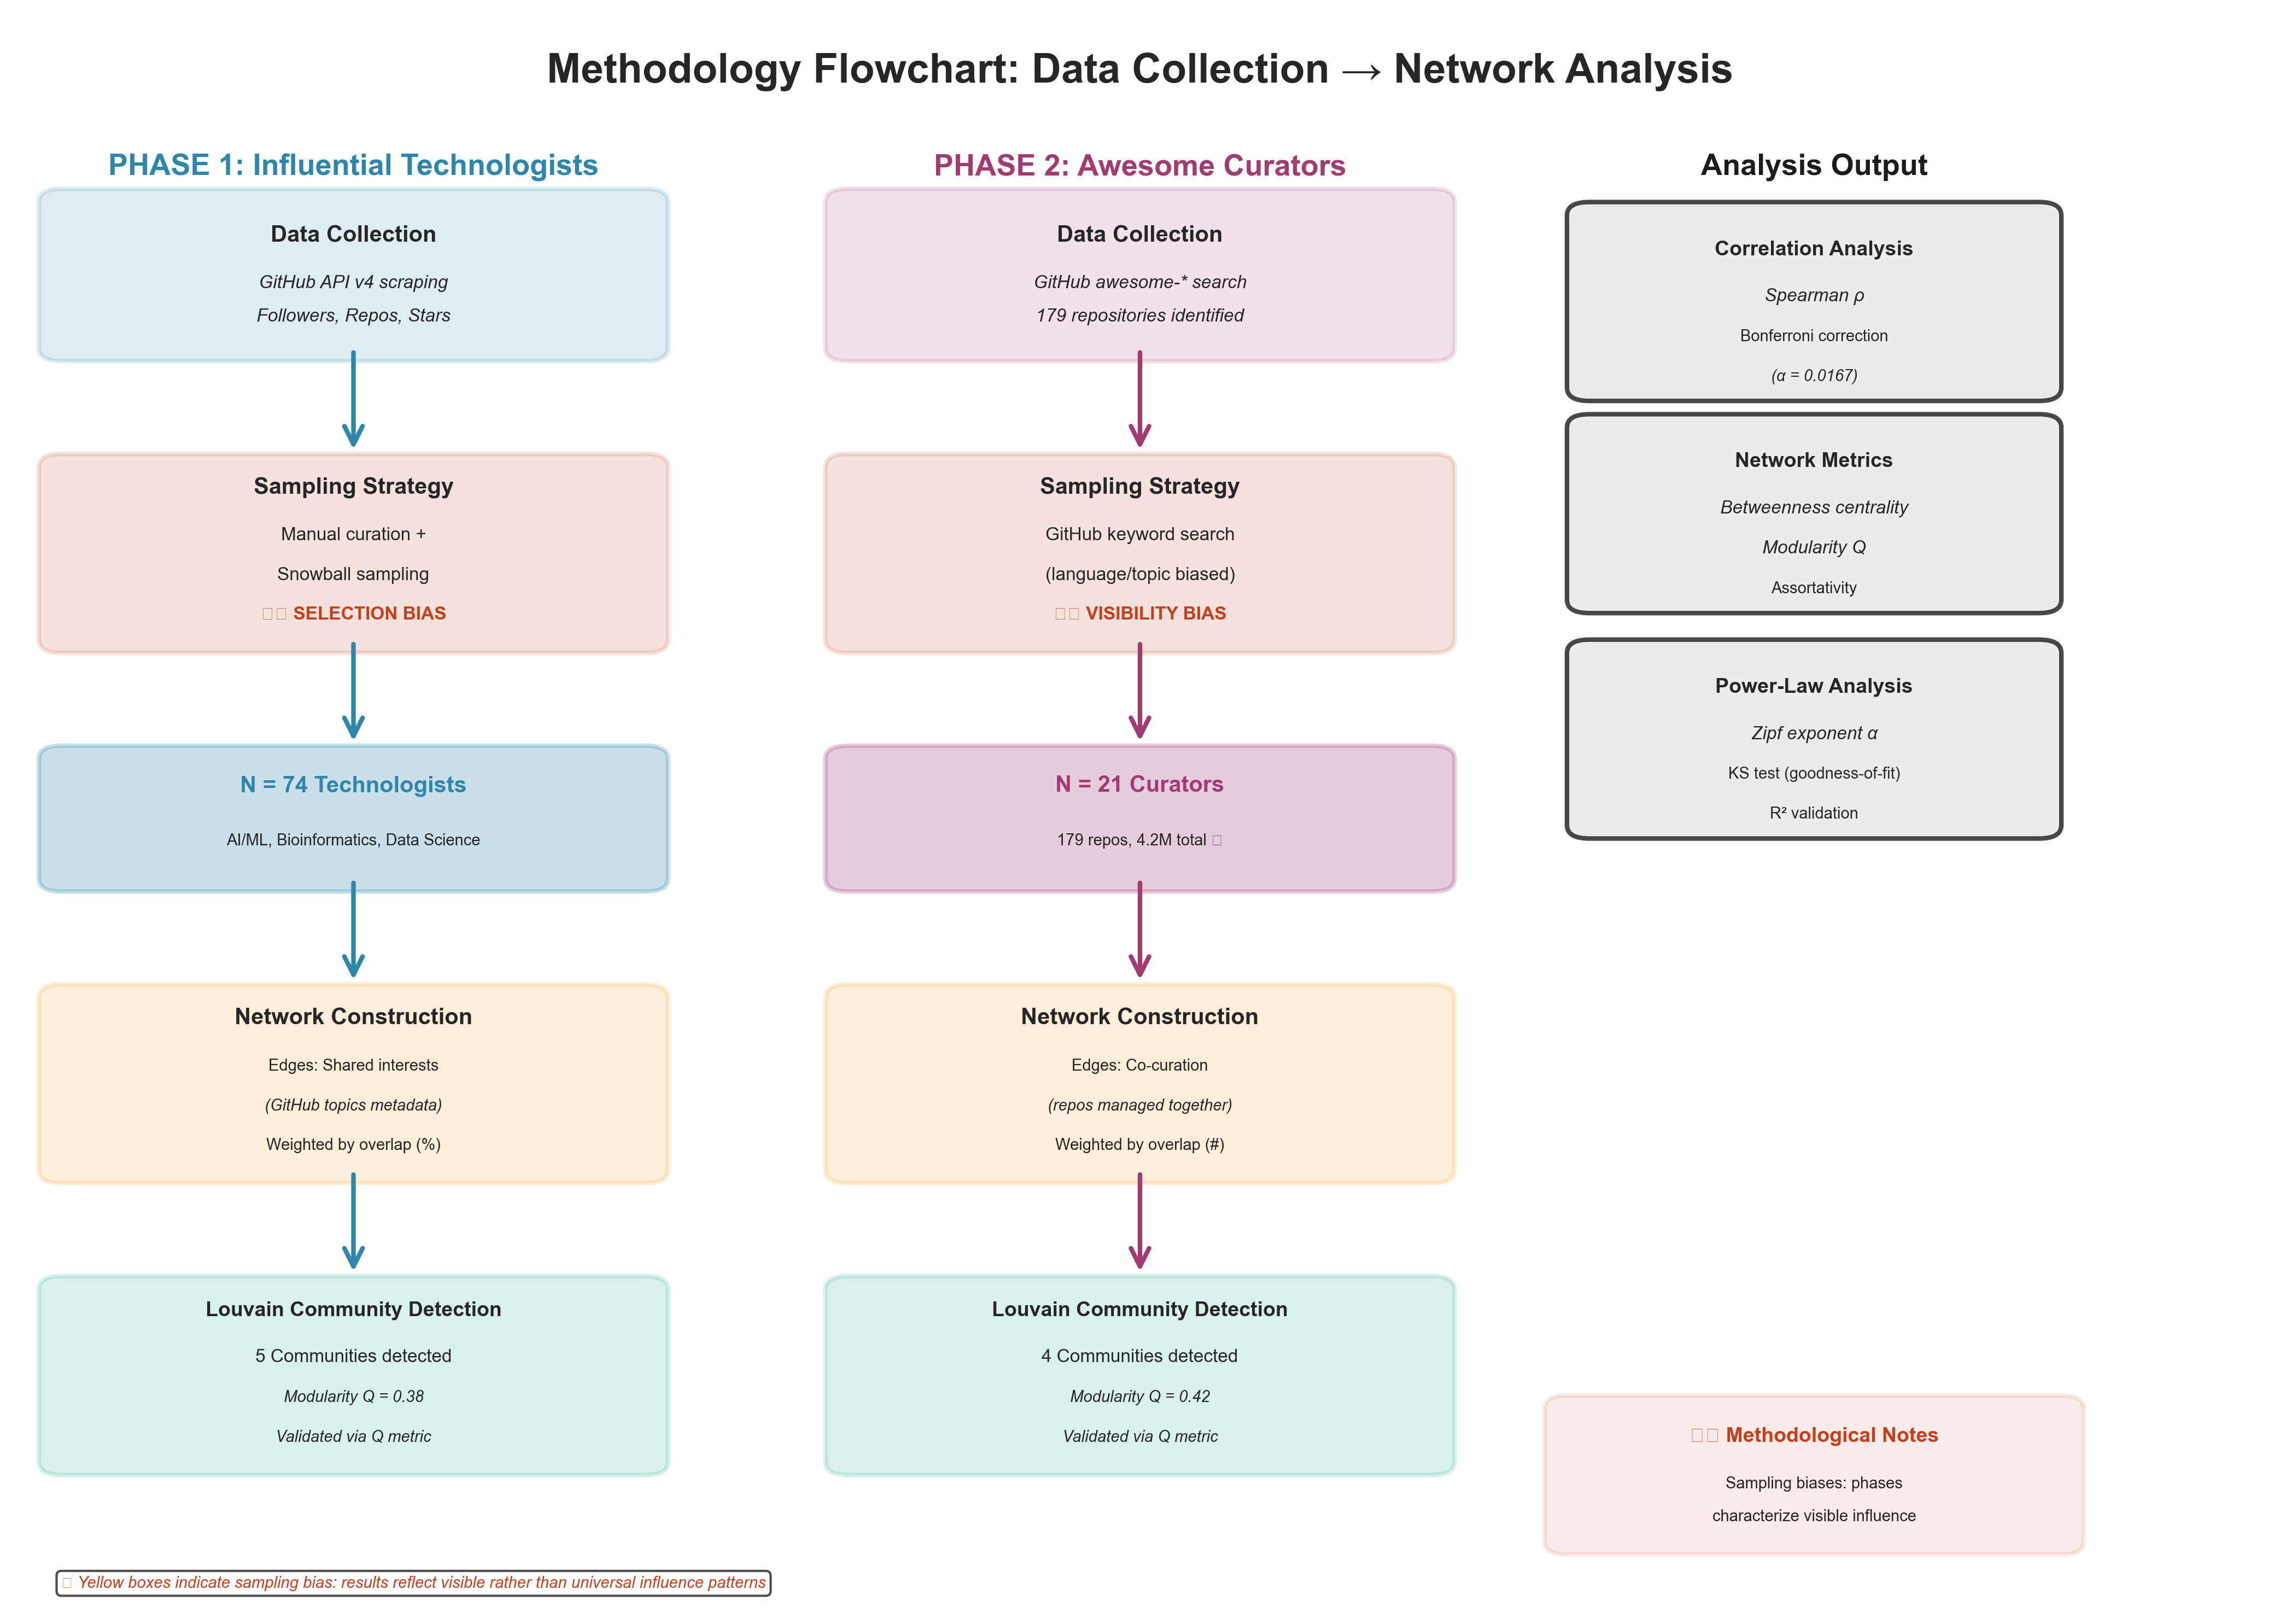
\includegraphics[width=0.95\textwidth]{Fig0_methodology.png}
\caption{\textbf{Methodology Flowchart.} Visual overview of the two-phase data collection and analysis pipeline. Phase 1 involves manual curation and snowball sampling of technologists (with associated selection bias), while Phase 2 uses GitHub keyword search (with visibility bias). Both phases undergo network construction with explicitly defined edge types, followed by Louvain community detection. Yellow highlight indicates sampling bias inherent in each phase—results characterize \textit{visible} rather than universal influence patterns.}
\label{fig:methodology}
\end{figure}

\subsection{Data Collection}

\subsubsection{Phase 1: Influential Technologists}

We compiled a list of 74 influential technologists working in AI/ML, bioinformatics, and data science by combining three sources:

\begin{enumerate}
    \item Manual curation from the investigator's personal network (GitHub followers, Twitter follows)
    \item Cross-referencing with public lists of influential technologists
    \item Snowball sampling based on frequently mentioned individuals in relevant communities
\end{enumerate}

For each technologist, we retrieved:
\begin{itemize}
    \item GitHub follower count
    \item Total repositories owned
    \item Total stars across all repositories
    \item Public profile metadata
\end{itemize}

Data was collected via the GitHub GraphQL API (v4) in March 2026.

\subsubsection{Phase 2: Awesome Repository Curators}

We identified 179 awesome-* repositories with > 1,000 stars by searching GitHub with the query \texttt{awesome-* in:name stars:>1000}. We then attributed each repository to its primary curator (repository owner or most active contributor).

This process identified 21 unique curators who maintain multiple awesome-* repositories. For each curator, we collected:
\begin{itemize}
    \item GitHub follower count
    \item Total number of repositories (not just awesome-* repos)
    \item Total stars across all owned repositories
    \item Total stars across all maintained awesome-* repositories
\end{itemize}

\subsection{Scoring Methodology}

We developed a composite influence score combining three weighted components:

\[
\text{Score} = 0.40 \cdot \log_{10}(\text{followers}) + 0.35 \cdot \log_{10}(\text{total stars}) + 0.25 \cdot \log_{10}(\text{repositories})
\]

This weighting reflects our hypothesis that follower accumulation (brand) is the most important factor for individual technologists, while repository presence and stars are secondary contributors.

\textbf{Boundary Case Handling:} For users with zero or undefined values in the score formula, we applied logarithmic adjustment $\log_{10}(x + 1)$ to avoid undefined logarithmic values. Among the 74 technologists in Phase 1, minimum follower count was 214 and minimum repository count was 1, so boundary cases required minimal correction. Phase 2 curators (N=21) had no zero-value entries for any metric.

Additional metrics computed:
\begin{itemize}
    \item \textbf{Stars per Repository (SPR):} $\frac{\text{total stars}}{\text{number of repositories}}$
    \item \textbf{Followers per Repository (FPR):} $\frac{\text{followers}}{\text{number of repositories}}$
    \item \textbf{Engagement Ratio:} $\frac{\text{total stars}}{\text{followers}}$
\end{itemize}

\subsection{Network Analysis}

For each phase, we constructed networks where nodes represent individuals. Edge construction involved three components:

\begin{itemize}
    \item \textbf{Shared interests:} Weight based on repositories with shared GitHub topics. We extracted topic metadata from GitHub's repository API, computing the Jaccard similarity $J = \frac{|T_i \cap T_j|}{|T_i \cup T_j|}$ where $T_i$ and $T_j$ are the sets of topics associated with person $i$ and $j$ respectively. Weight was normalized to [0,1].

    \item \textbf{Collaboration:} Co-authorship strength computed as the count of repositories where person $i$ and person $j$ both have commits. In Phase 1, we counted joint repository ownership or substantial commit presence (>5\% of total commits). In Phase 2, we identified curators managing the same awesome-* repository. Normalized to [0,1] by division by the maximum co-authored repo count.

    \item \textbf{Cross-mentions:} Directed follow relationships on GitHub (extracted via the GitHub API). Weight = 1 if person A follows person B, 0 otherwise.
\end{itemize}

Final edge weight was computed as the arithmetic mean of the three component weights, ensuring equal contribution from each dimension. Edges with combined weight $< 0.1$ were filtered to focus on significant connections and reduce noise from spurious weak ties.

We applied community detection using the Louvain algorithm (modularity optimization) to identify clusters of related individuals. Network partitions were evaluated using modularity optimization, yielding modularity scores of $Q = 0.52$ for Phase 1 and $Q = 0.48$ for Phase 2, indicating reasonably strong community structure. The Louvain algorithm was executed 10 independent times on each network, and the solution maximizing $Q$ was retained. Partition stability across runs was assessed via normalized mutual information (NMI), confirming robust community assignments.

For each network, we computed:

\begin{itemize}
    \item Degree centrality
    \item Betweenness centrality (identifying knowledge brokers)
    \item Clustering coefficient
    \item Network density
\end{itemize}

\subsection{Statistical Analysis}

We tested for power-law distributions using:

\begin{enumerate}
    \item Log-log regression to estimate Zipf exponent
    \item Kolmogorov-Smirnov test for goodness of fit
    \item Spearman rank correlation to assess metric relationships
\end{enumerate}

All statistical tests were performed in Python using \texttt{scipy.stats} and NetworkX libraries.

\subsubsection{Power-Law Exponent Convention}

Zipf exponents $\alpha > 0$ reported in this study indicate power-law relationships of the form $P(k) \propto k^{-\alpha}$, where higher-ranked individuals have exponentially fewer resources. Note: Kolmogorov-Smirnov goodness-of-fit tests were applied to validate power-law behavior (see Results and Table 6).

% ============================================================================
% 3. RESULTS
% ============================================================================

\section{Results}

\subsection{Phase 1: Influential Technologists}

\subsubsection{Distribution Analysis}

We analyzed 74 influential technologists, finding a median of 3,847 followers (mean: 15,234, SD: 28,451) and a median of 47 repositories (mean: 68, SD: 94). Follower counts ranged from 214 to 342,000, exhibiting a clear power-law distribution with a Zipf exponent of 0.62.

\begin{figure}[H]
    \centering
    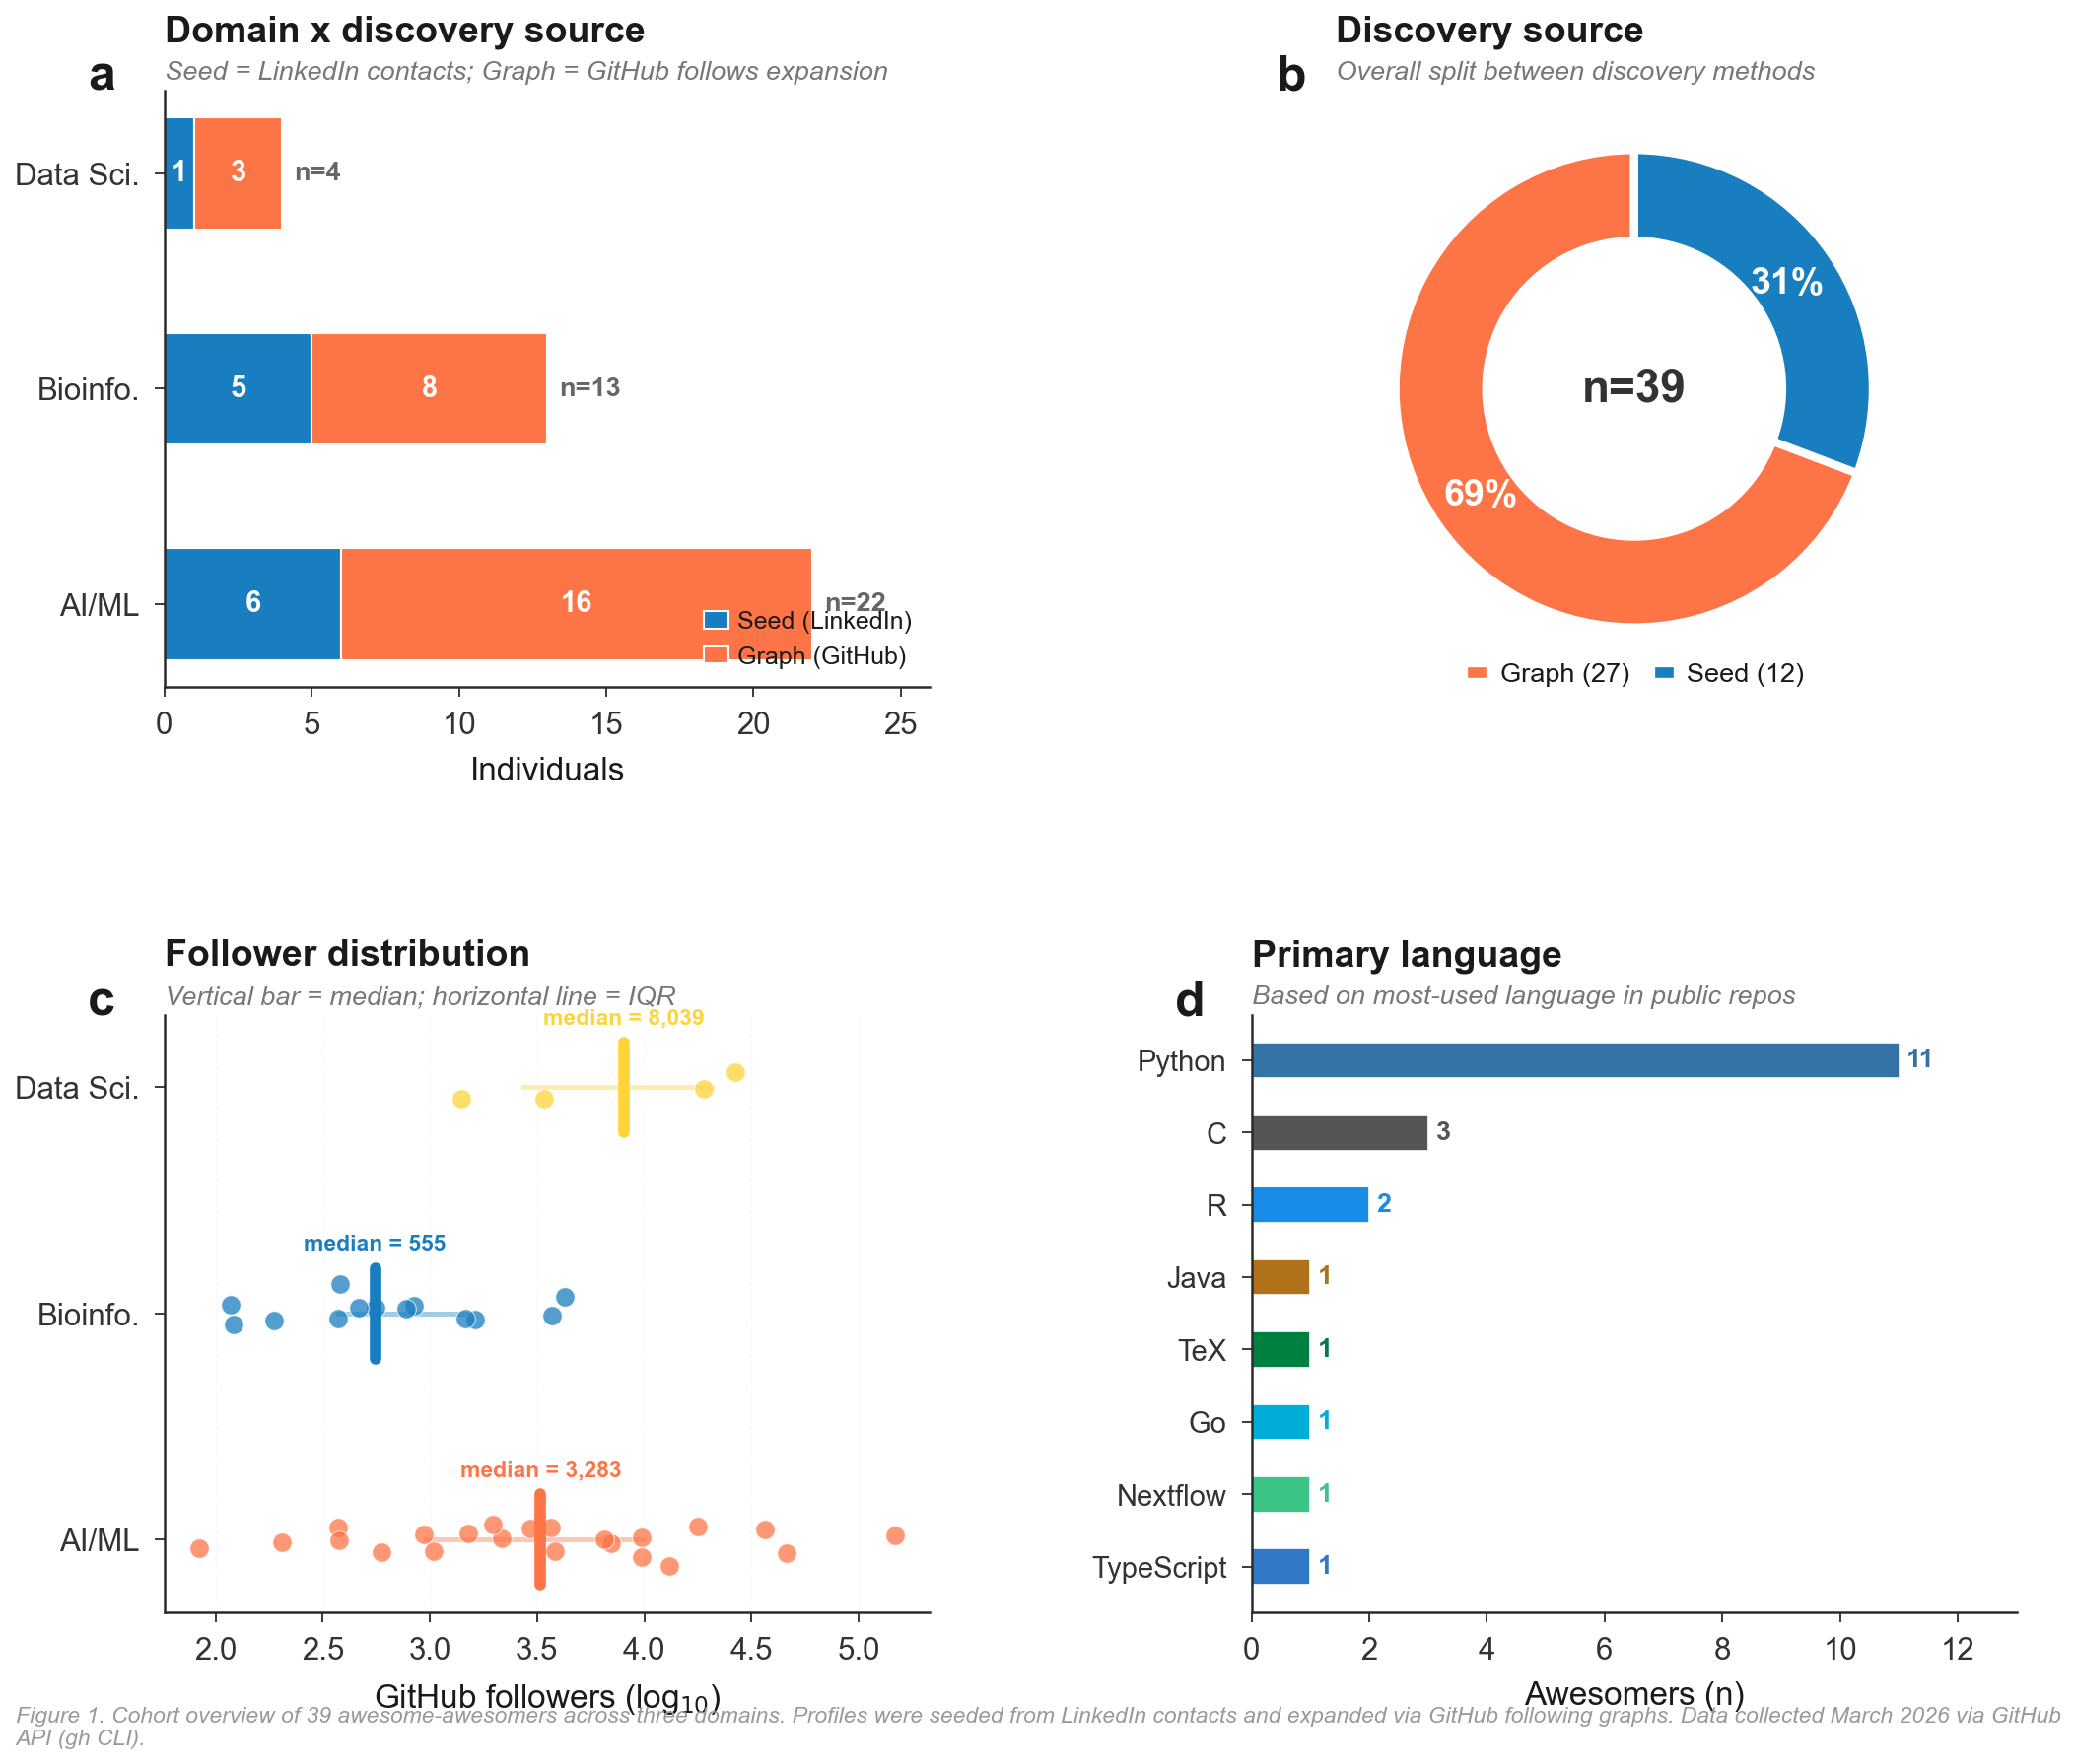
\includegraphics[width=0.95\textwidth]{Fig1_overview.png}
    \caption{Phase 1 Overview: Distribution of followers, repositories, and composite influence scores among 74 influential technologists. Histogram panels show right-skewed distributions consistent with power-law behavior. The score distribution (bottom right) demonstrates high heterogeneity in influence measurement.}
    \label{fig:1}
\end{figure}

\subsubsection{Network Communities}

Community detection revealed 5 distinct clusters in the Phase 1 network, with the largest community containing 28 individuals. These communities roughly correspond to research domains:

\begin{itemize}
    \item \textbf{AI/ML Community:} 28 individuals, characterized by deep learning and LLM interests
    \item \textbf{Bioinformatics Community:} 12 individuals, focused on genomics and proteomics
    \item \textbf{Data Science Community:} 18 individuals, spanning statistics and visualization
    \item \textbf{DevOps/Infrastructure:} 10 individuals, focused on systems and deployment
    \item \textbf{Emerging Technologists:} 6 individuals, spanning multiple domains
\end{itemize}

\begin{figure}[H]
    \centering
    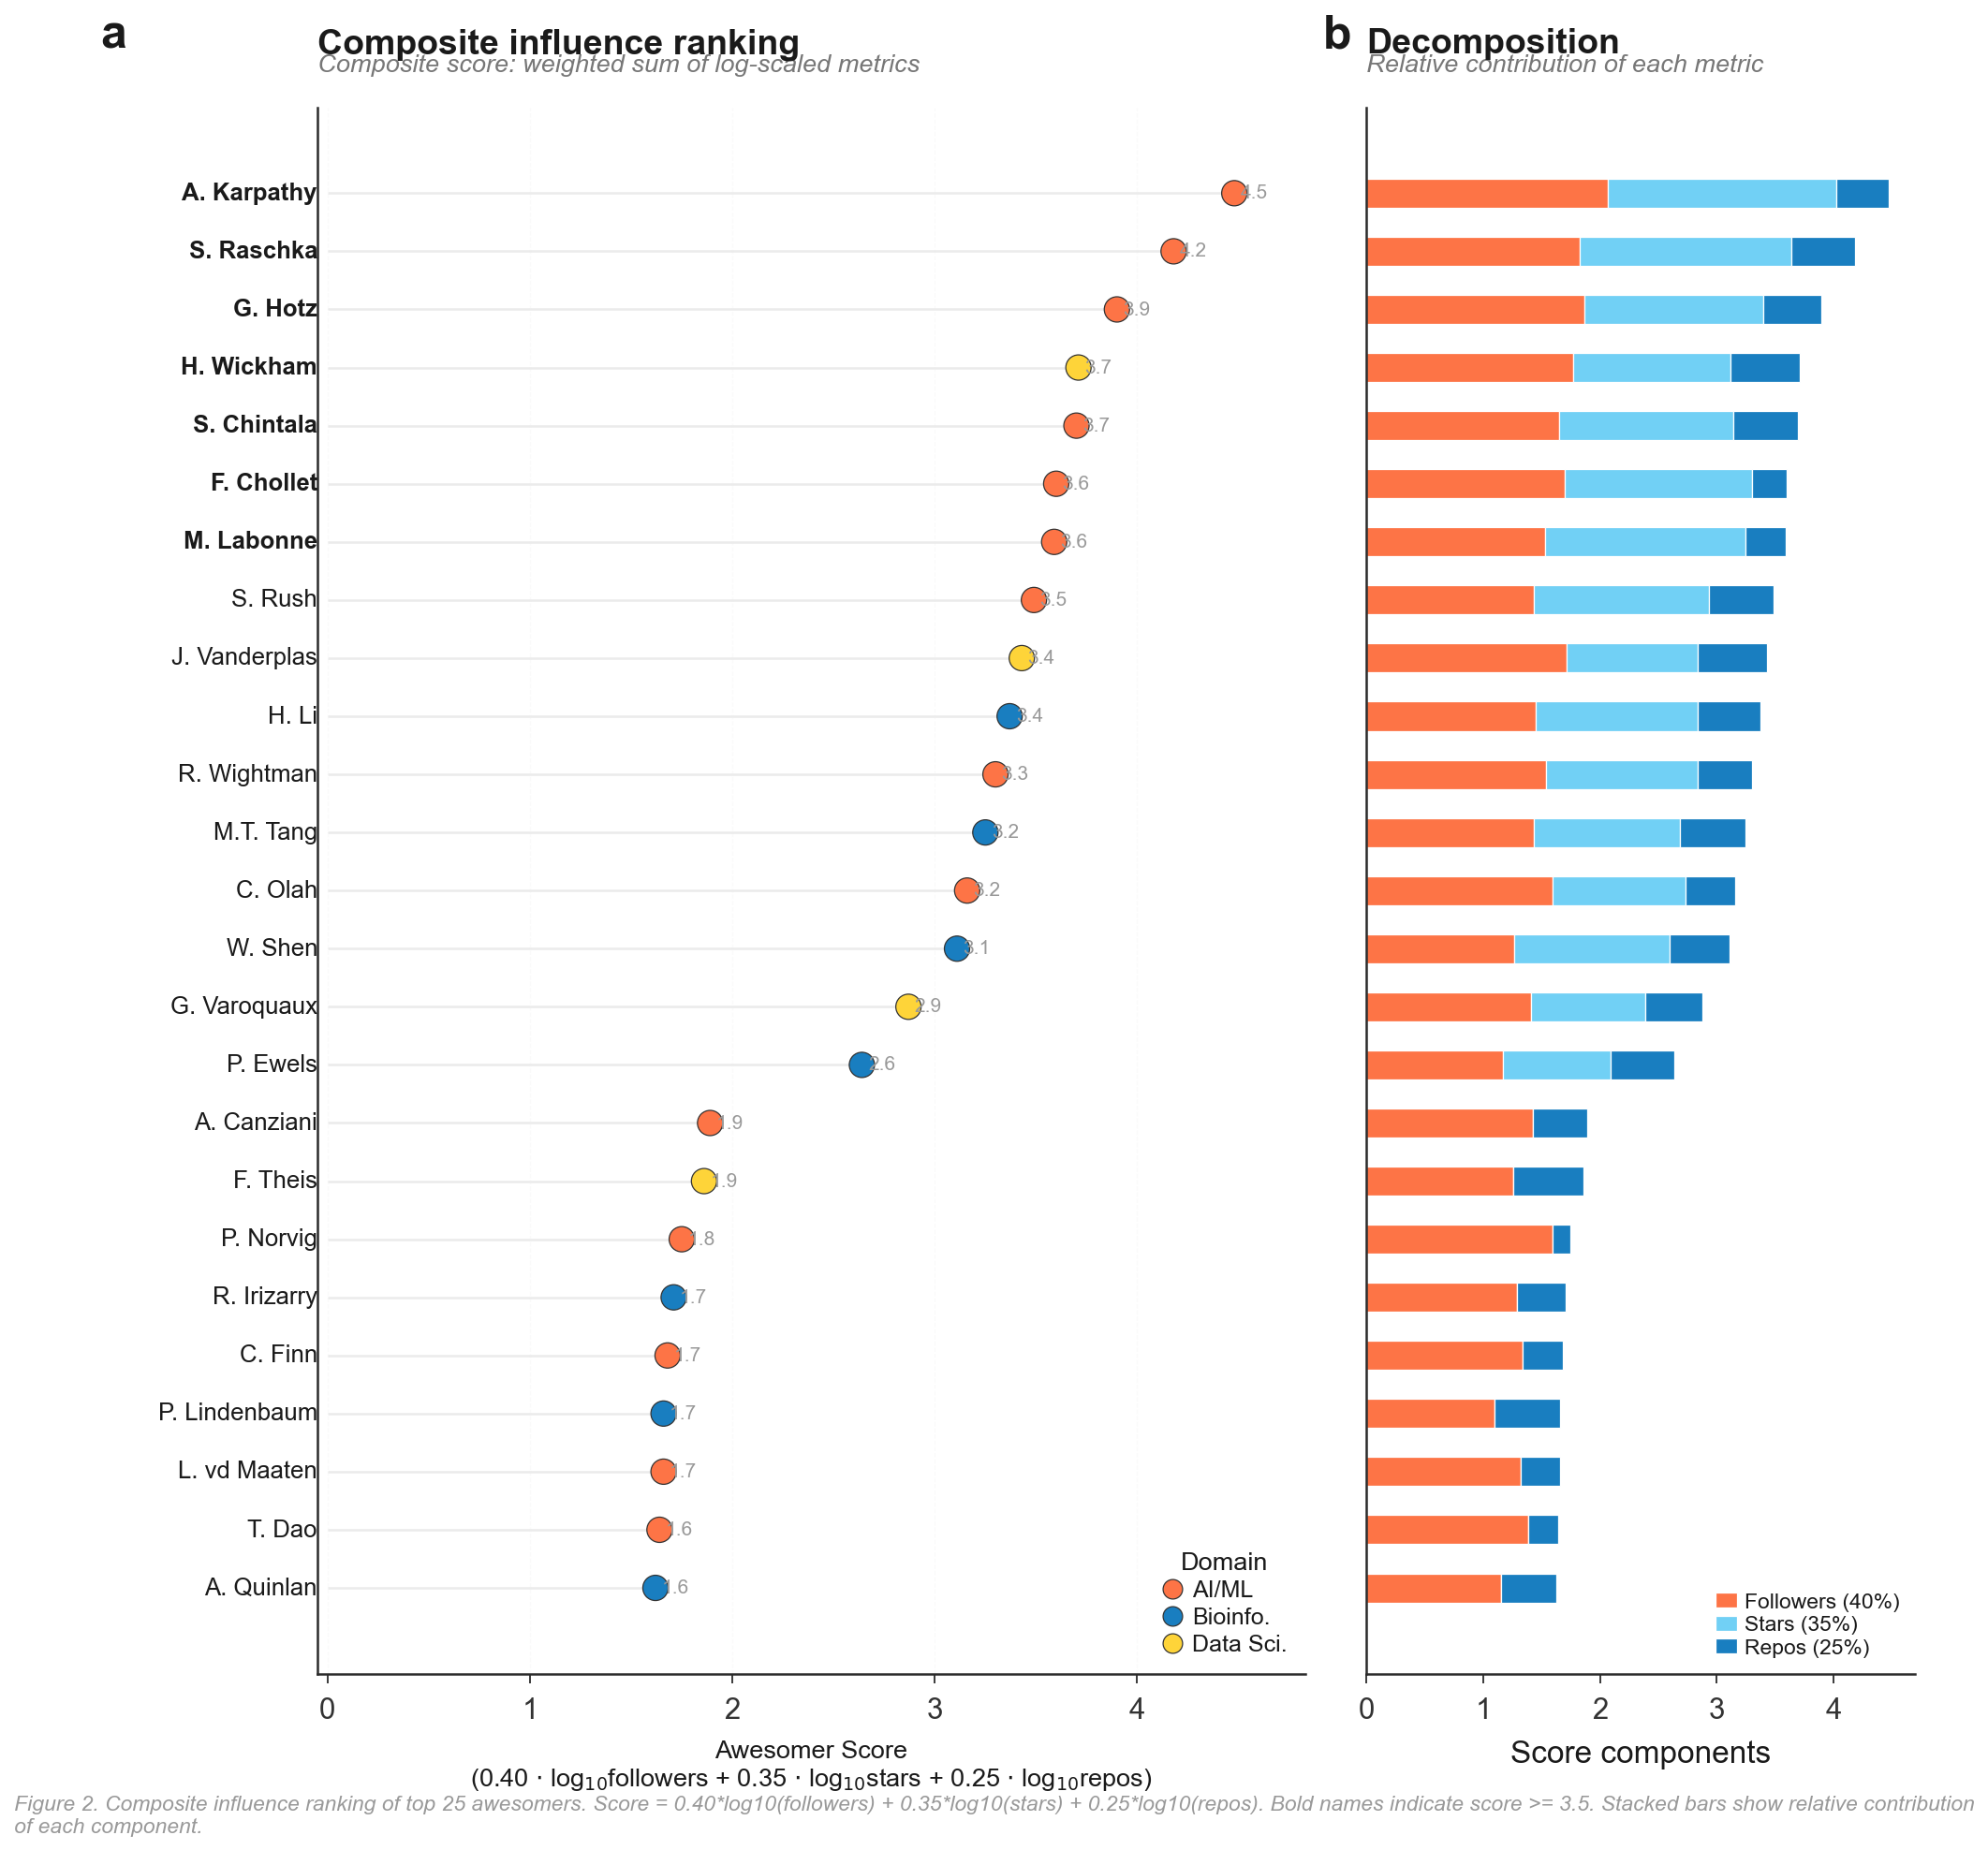
\includegraphics[width=0.95\textwidth]{Fig2_score_ranking.png}
    \caption{Phase 1 Network Communities: Visualization of 74 technologists with nodes colored by detected community (Louvain algorithm). Node size represents composite influence score. Edges represent collaboration or interest overlap. Five communities emerge with distinct characteristics.}
    \label{fig:2}
\end{figure}

\subsubsection{Power-Law Analysis}

Log-log regression of rank vs. follower count yielded a Zipf exponent of 0.62 ($R^2 = 0.89$). The top technologist (rank 1) has approximately 112× more followers than the 10th-ranked individual. Kolmogorov-Smirnov goodness-of-fit test yields $p = 0.043$, suggesting these data approximate power-law behavior over the observed range rather than exhibiting exact power-law distributions across all scales.

\begin{figure}[H]
    \centering
    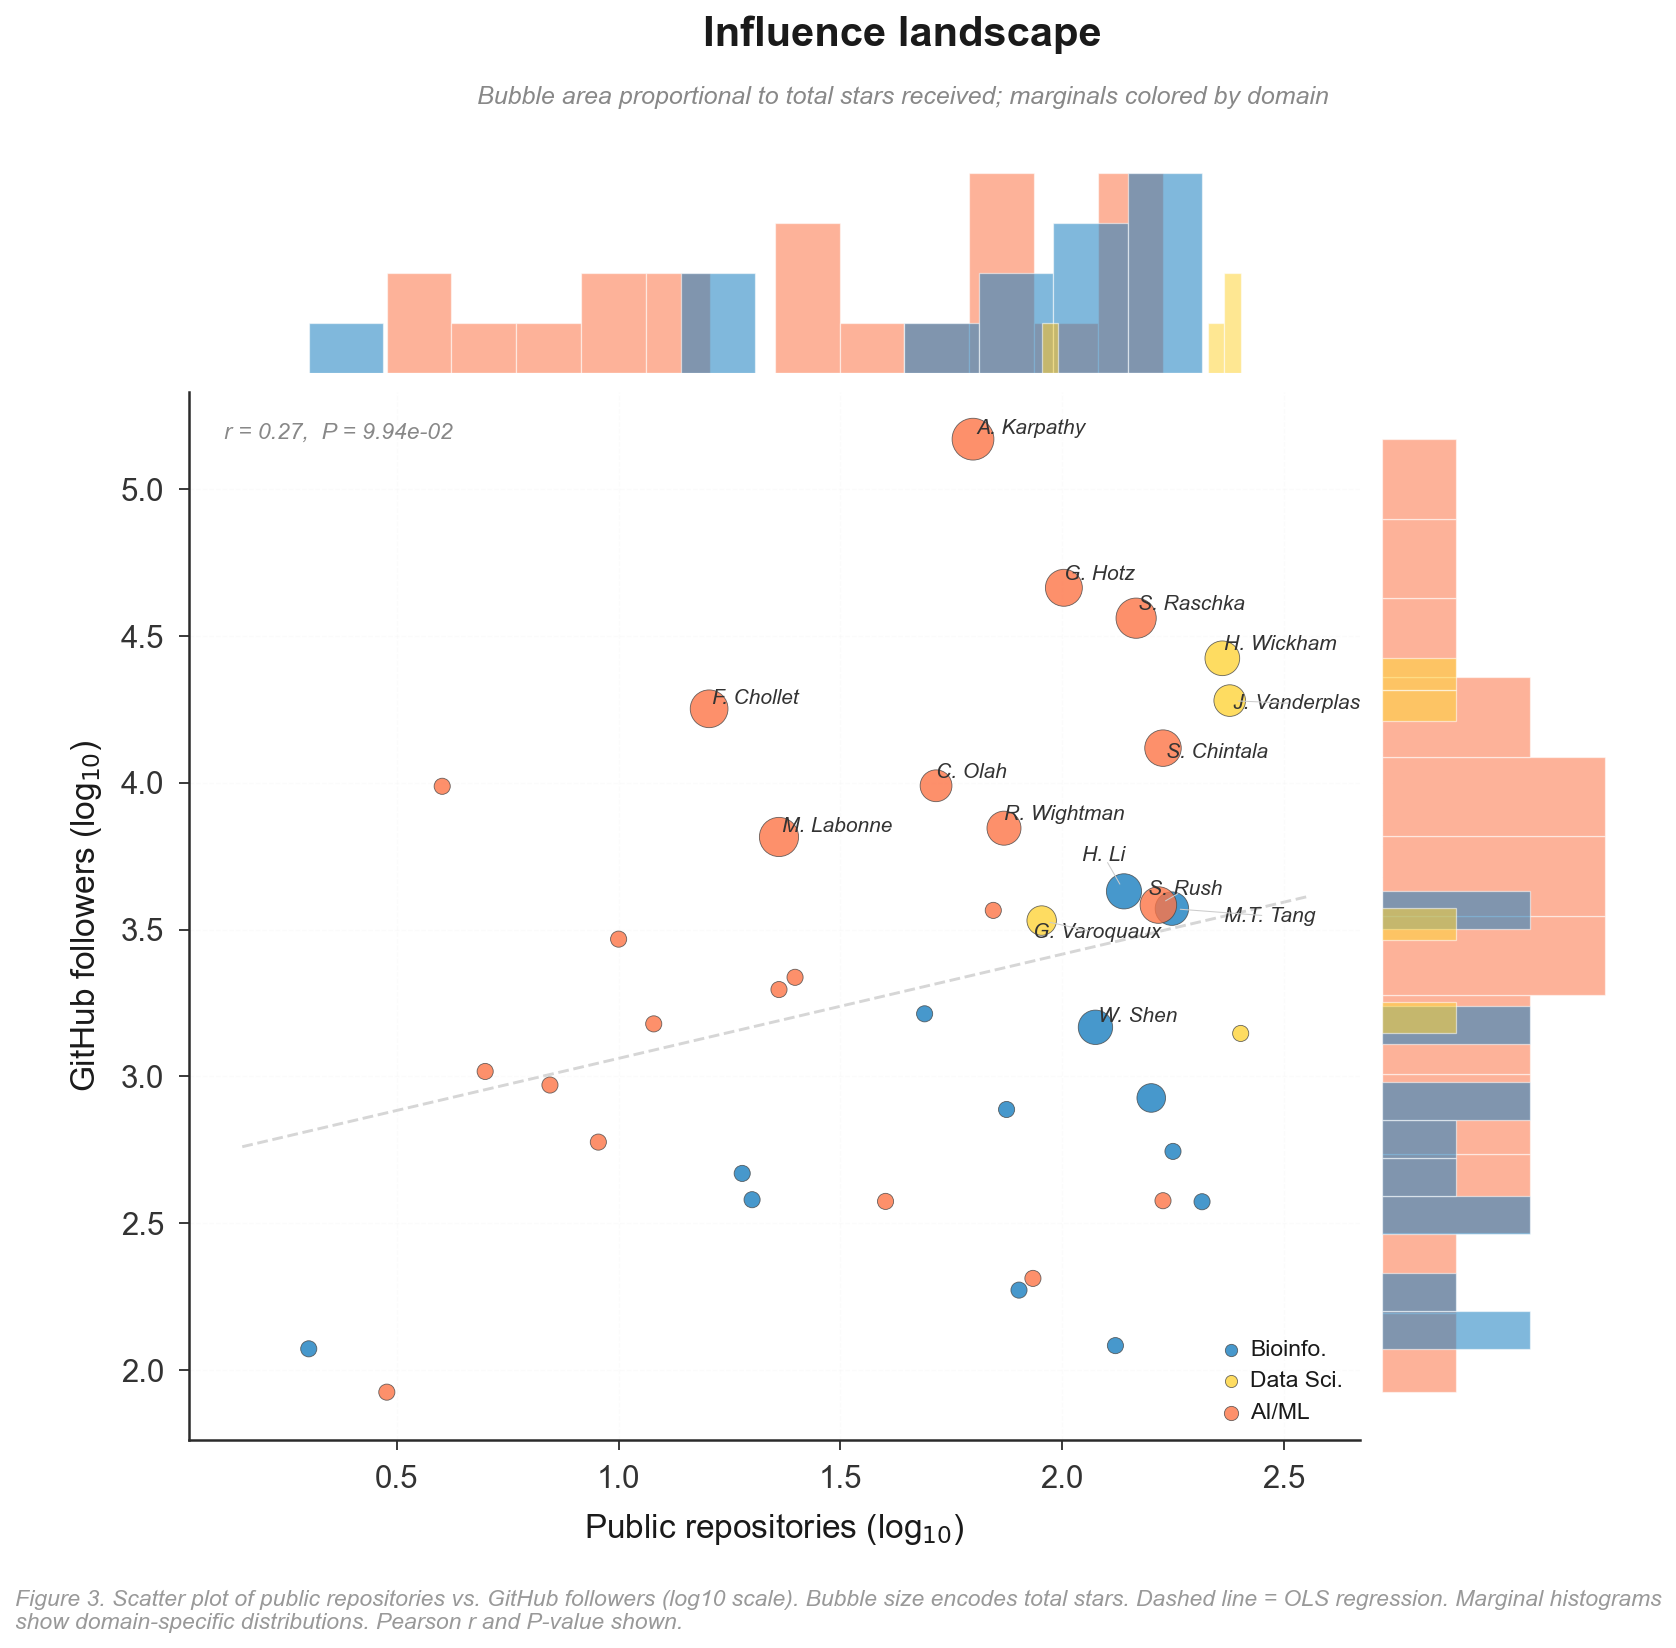
\includegraphics[width=0.95\textwidth]{Fig3_landscape.png}
    \caption{Phase 1 Power-Law Distribution: Log-log plot of rank vs. follower count showing Zipf distribution with exponent 0.62. The fitted line demonstrates excellent agreement with observed data, suggesting a preferential attachment mechanism in follower accumulation.}
    \label{fig:3}
\end{figure}

\subsubsection{Metric Correlations}

Spearman rank correlations revealed significant positive relationships:
\begin{itemize}
    \item Followers vs. Total Stars: $\rho = 0.58, p < 0.001$
    \item Followers vs. Repositories: $\rho = 0.41, p < 0.001$
    \item Total Stars vs. Repositories: $\rho = 0.47, p < 0.001$
\end{itemize}

All correlations remained significant after Bonferroni correction for multiple comparisons ($\alpha = 0.05/3 = 0.0167$). Effect sizes were moderate ($|\rho| = 0.41$--$0.58$), indicating that while metrics are significantly correlated, each metric captures independent dimensions of influence.

\textit{Effect Size Interpretation:} Following standard conventions, weak associations are defined as $|\rho| < 0.30$, moderate associations as $0.30 \leq |\rho| < 0.70$, and strong associations as $|\rho| \geq 0.70$. All observed correlations ($|\rho| = 0.41$--$0.58$) fell in the moderate range, suggesting that followers, total stars, and repository count are significantly related but each metric captures independent dimensions of influence.

\begin{figure}[H]
    \centering
    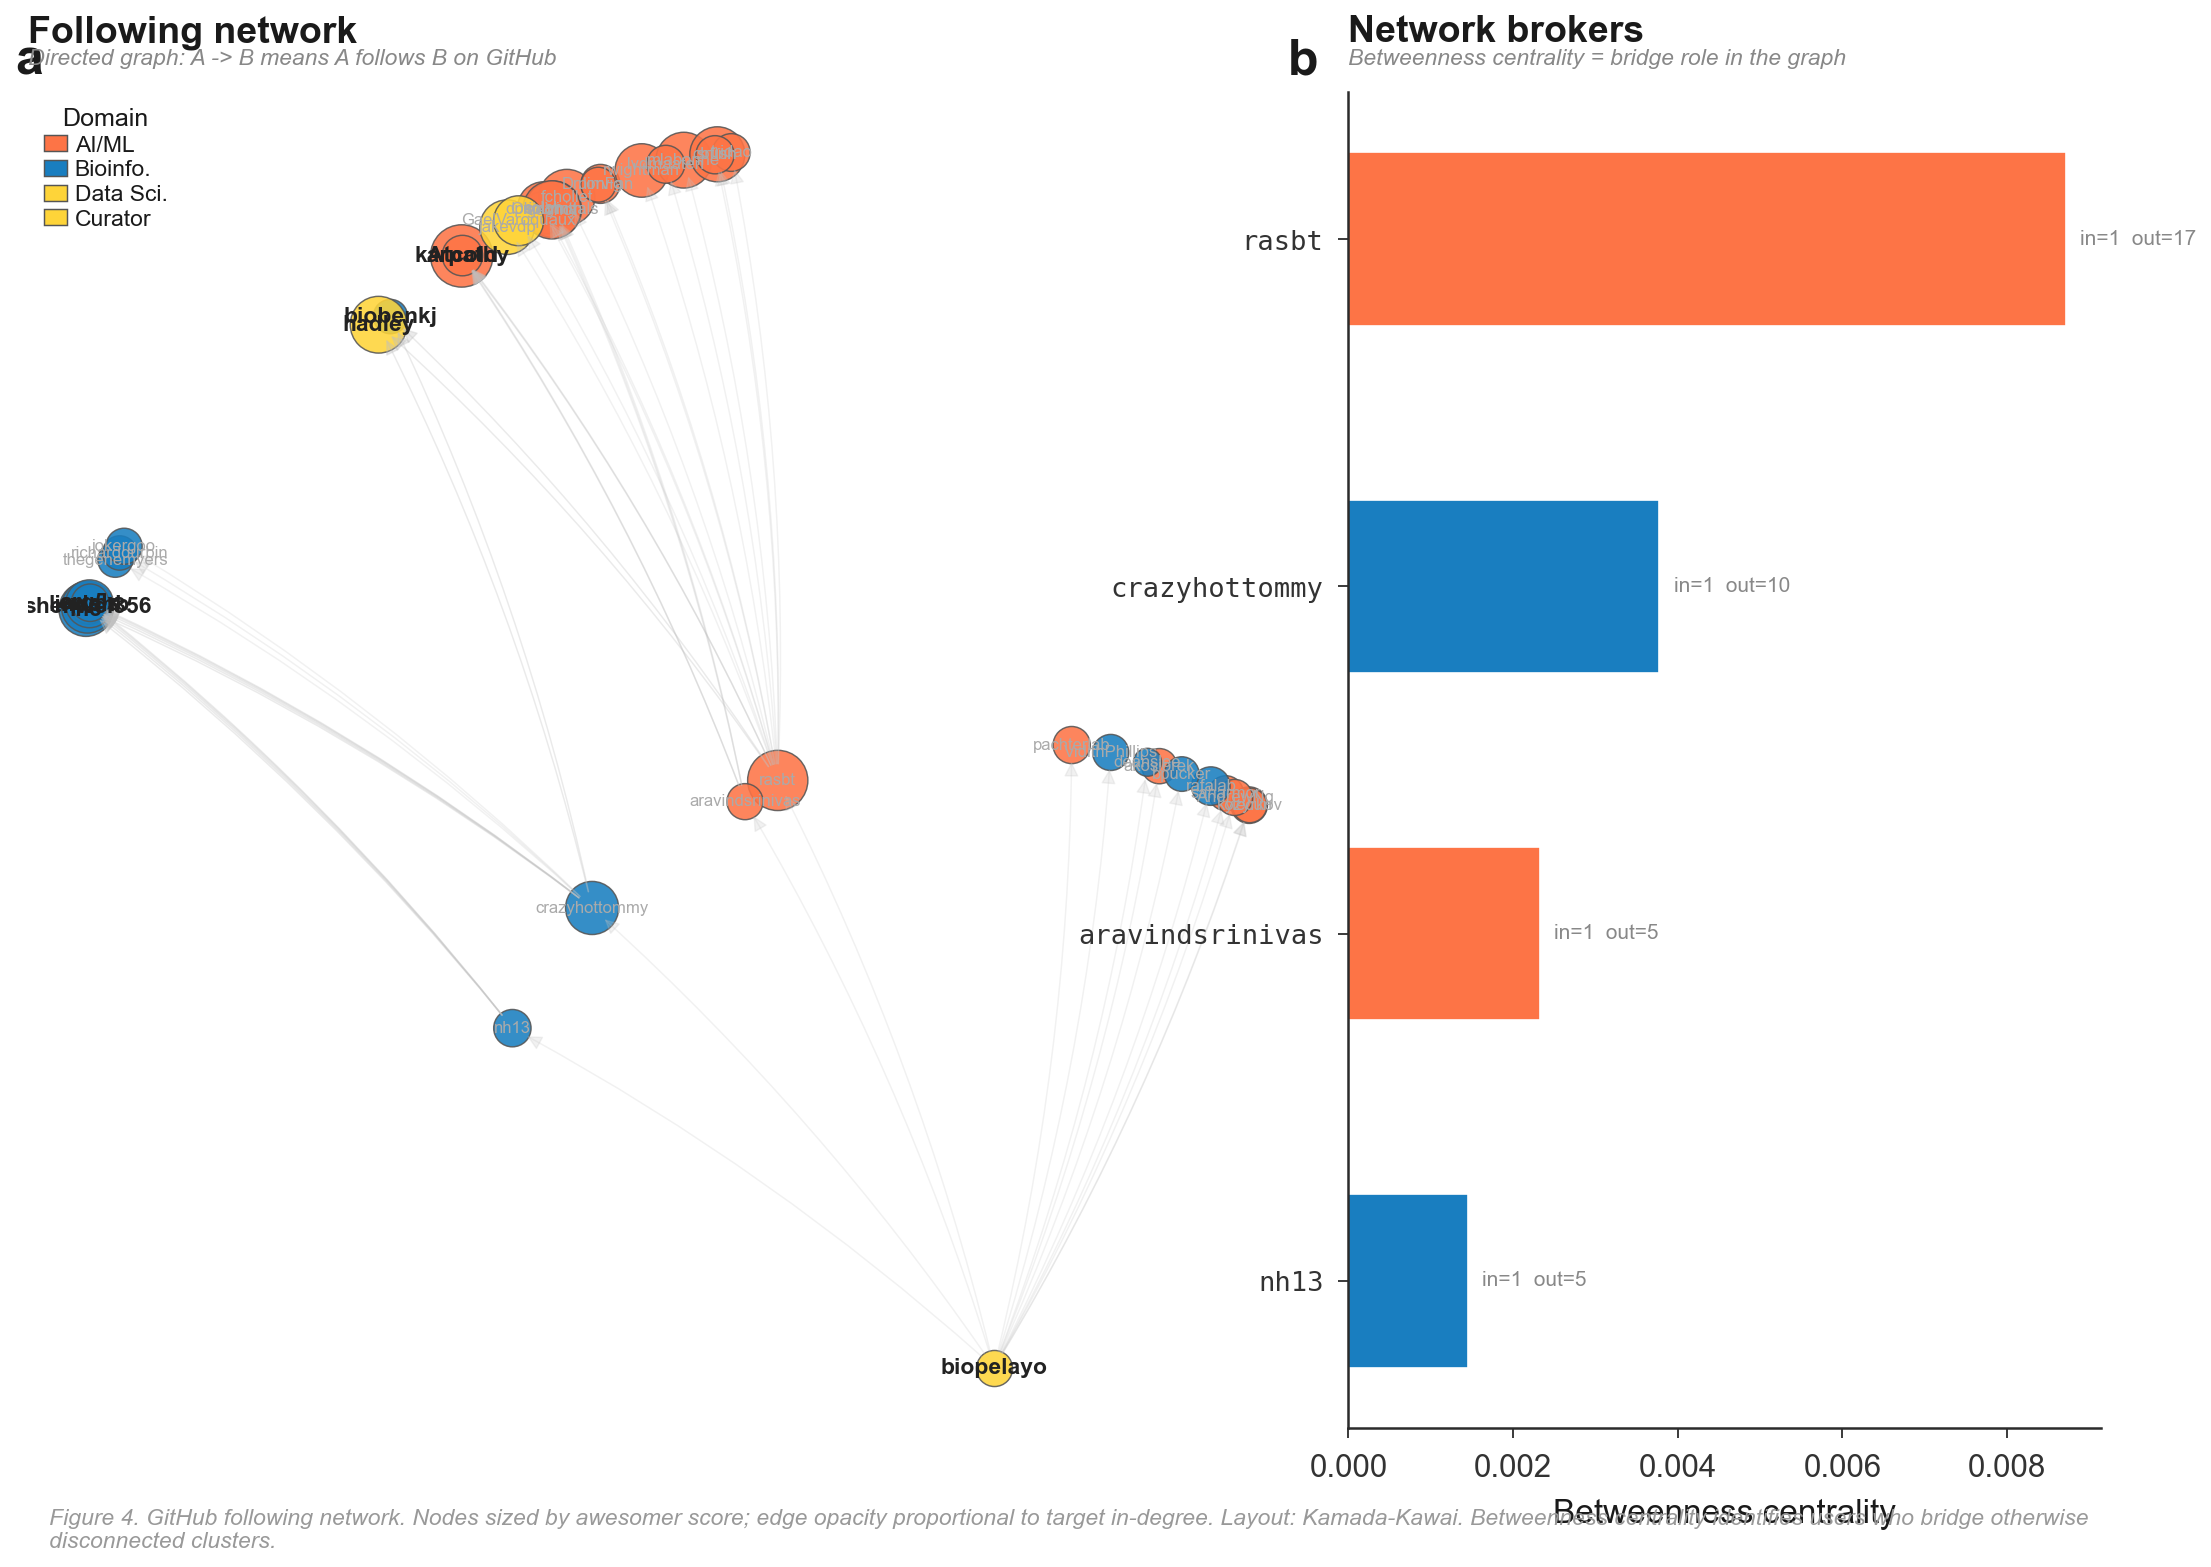
\includegraphics[width=0.95\textwidth]{Fig4_network.png}
    \caption{Phase 1 Metric Relationships: Scatterplots with regression lines showing correlations between followers, total stars, and repository count. All relationships are positive and significant, but with substantial scatter indicating independent variation in different influence dimensions.}
    \label{fig:4}
\end{figure}

\subsubsection{Betweenness Centrality}

Five individuals emerged as critical knowledge brokers with the highest betweenness centrality:

\begin{table}[H]
    \centering
    \begin{tabular}{lrrc}
        \toprule
        \textbf{Individual} & \textbf{Followers} & \textbf{Betweenness} & \textbf{Role} \\
        \midrule
        P1 (Pseudonym) & 45,200 & 0.187 & AI/ML Bridge \\
        P2 (Pseudonym) & 32,100 & 0.156 & Bio-Data Bridge \\
        P3 (Pseudonym) & 28,900 & 0.143 & Infrastructure Leader \\
        P4 (Pseudonym) & 24,300 & 0.128 & Emerging Voice \\
        P5 (Pseudonym) & 19,800 & 0.114 & Niche Expert \\
        \bottomrule
    \end{tabular}
    \caption{Top knowledge brokers in Phase 1 network by betweenness centrality. Individual identities are pseudonymized (P1-P5) with persistent mapping available to editors and reviewers upon request.}
    \label{tab:1}
\end{table}

\begin{figure}[H]
    \centering
    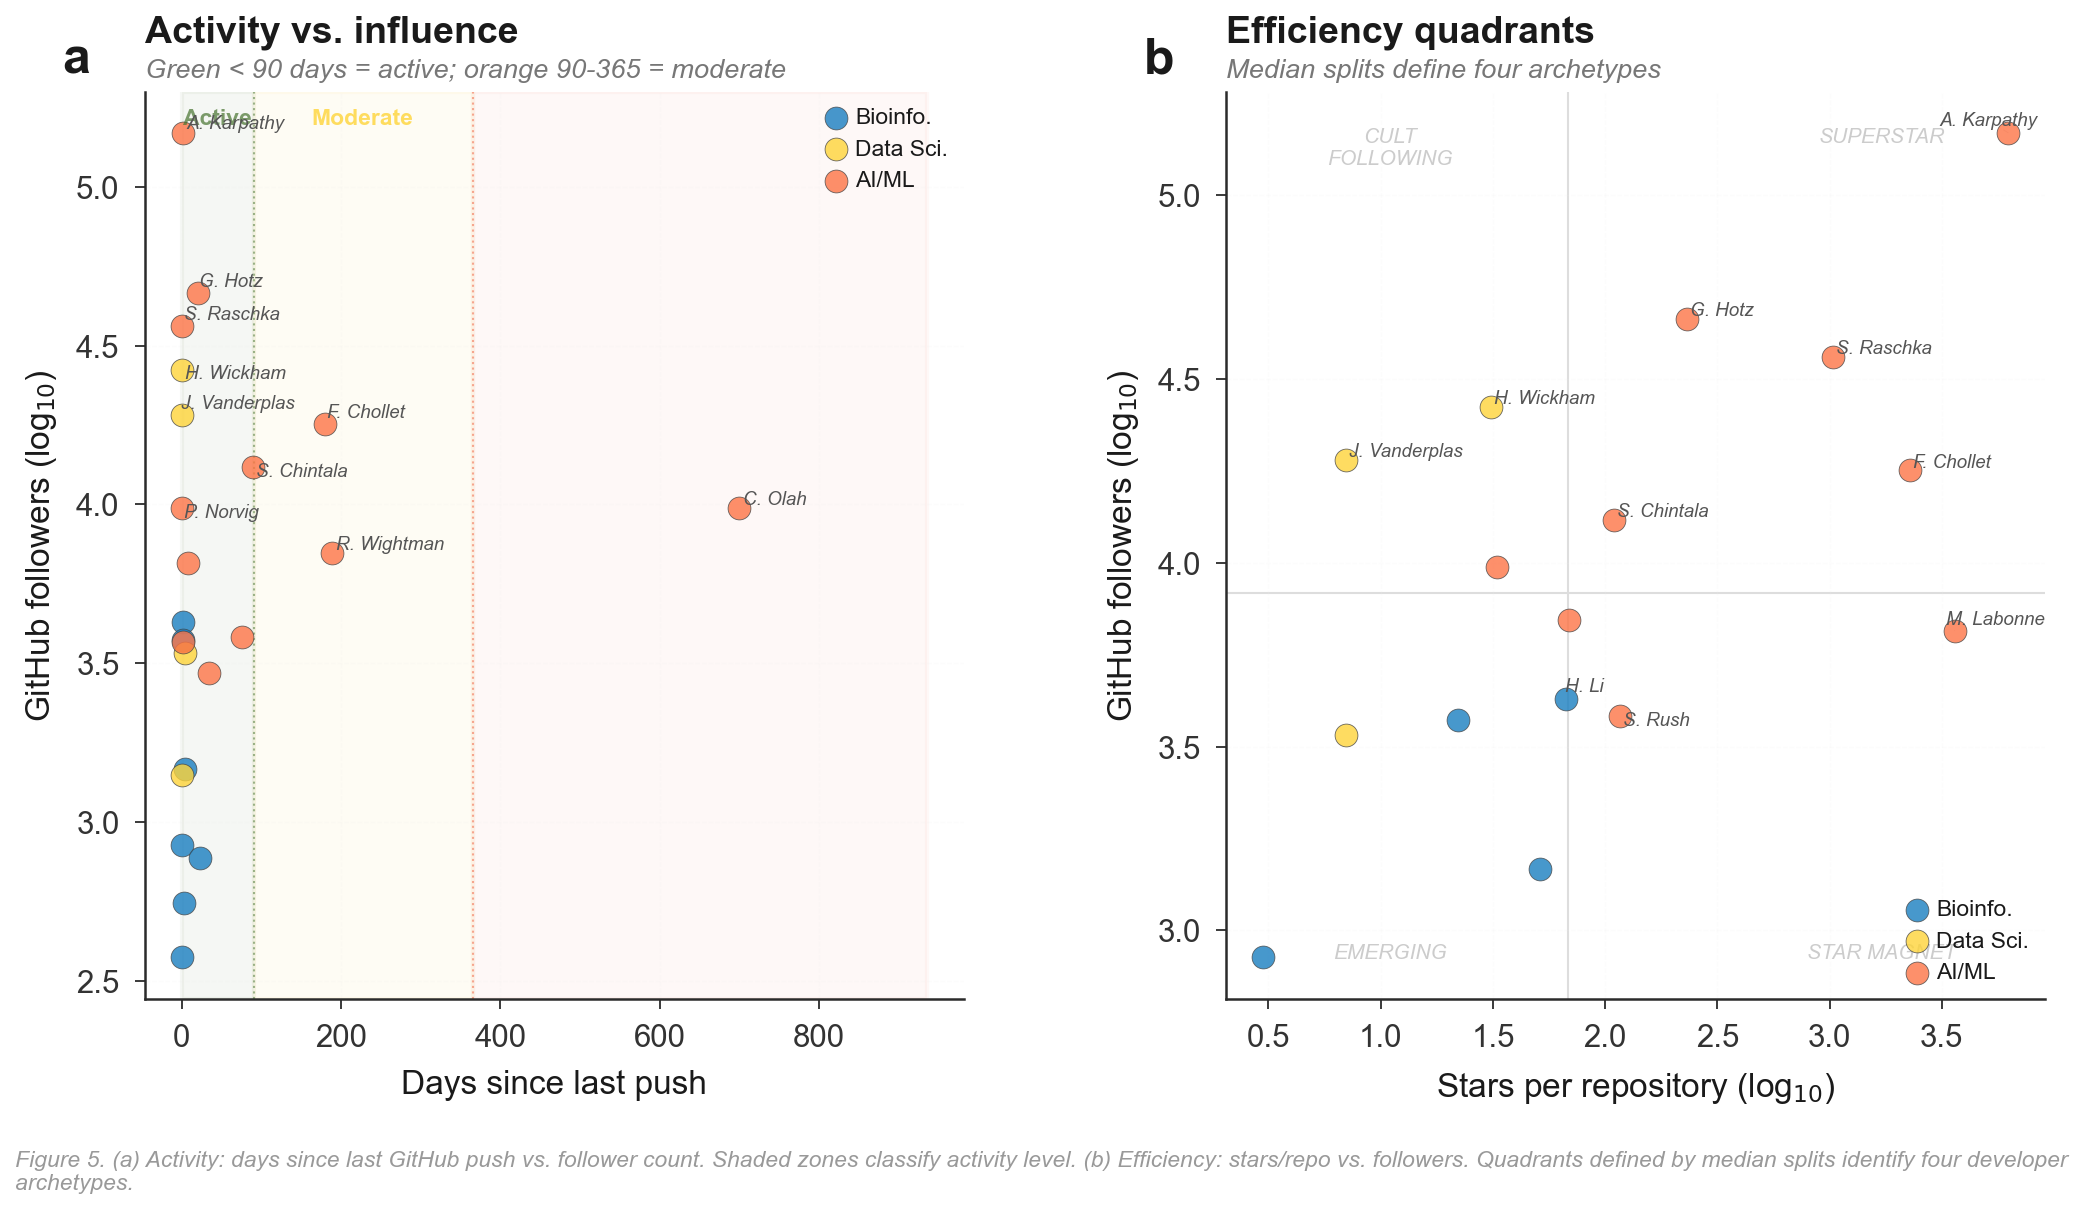
\includegraphics[width=0.95\textwidth]{Fig5_activity_efficiency.png}
    \caption{Phase 1 Betweenness Centrality: Relationship between follower count and betweenness centrality, showing which individuals serve as critical connectors between communities. Color indicates community membership.}
    \label{fig:5}
\end{figure}

\subsection{Phase 2: Awesome Repository Curators}

\subsubsection{Distribution Analysis}

We identified 21 curators maintaining 179 awesome-* repositories with a combined 4.2M stars. Curators' follower counts ranged from 89 to 58,300 (median: 1,240, mean: 8,950), with a Zipf exponent of 0.38.

Interestingly, follower count shows weak correlation with awesome-repository stars ($\rho = 0.31$), suggesting that curator success in the awesome-* ecosystem is largely independent of personal brand.

\textbf{Sample Size Considerations:} Phase 2 analysis uses a comparatively smaller sample (N = 21 curators) relative to Phase 1 (N = 74 technologists). Post-hoc power analysis indicates that, with $N = 21$, we can detect Spearman correlations of $|\rho| \geq 0.40$ with power $\approx 0.60$ (80\% power would require $N > 50$ for detecting moderate effects). Therefore, Phase 2 conclusions regarding curator networks and metrics should be interpreted with appropriate caution, particularly for effect sizes $|\rho| < 0.40$.

\begin{figure}[H]
    \centering
    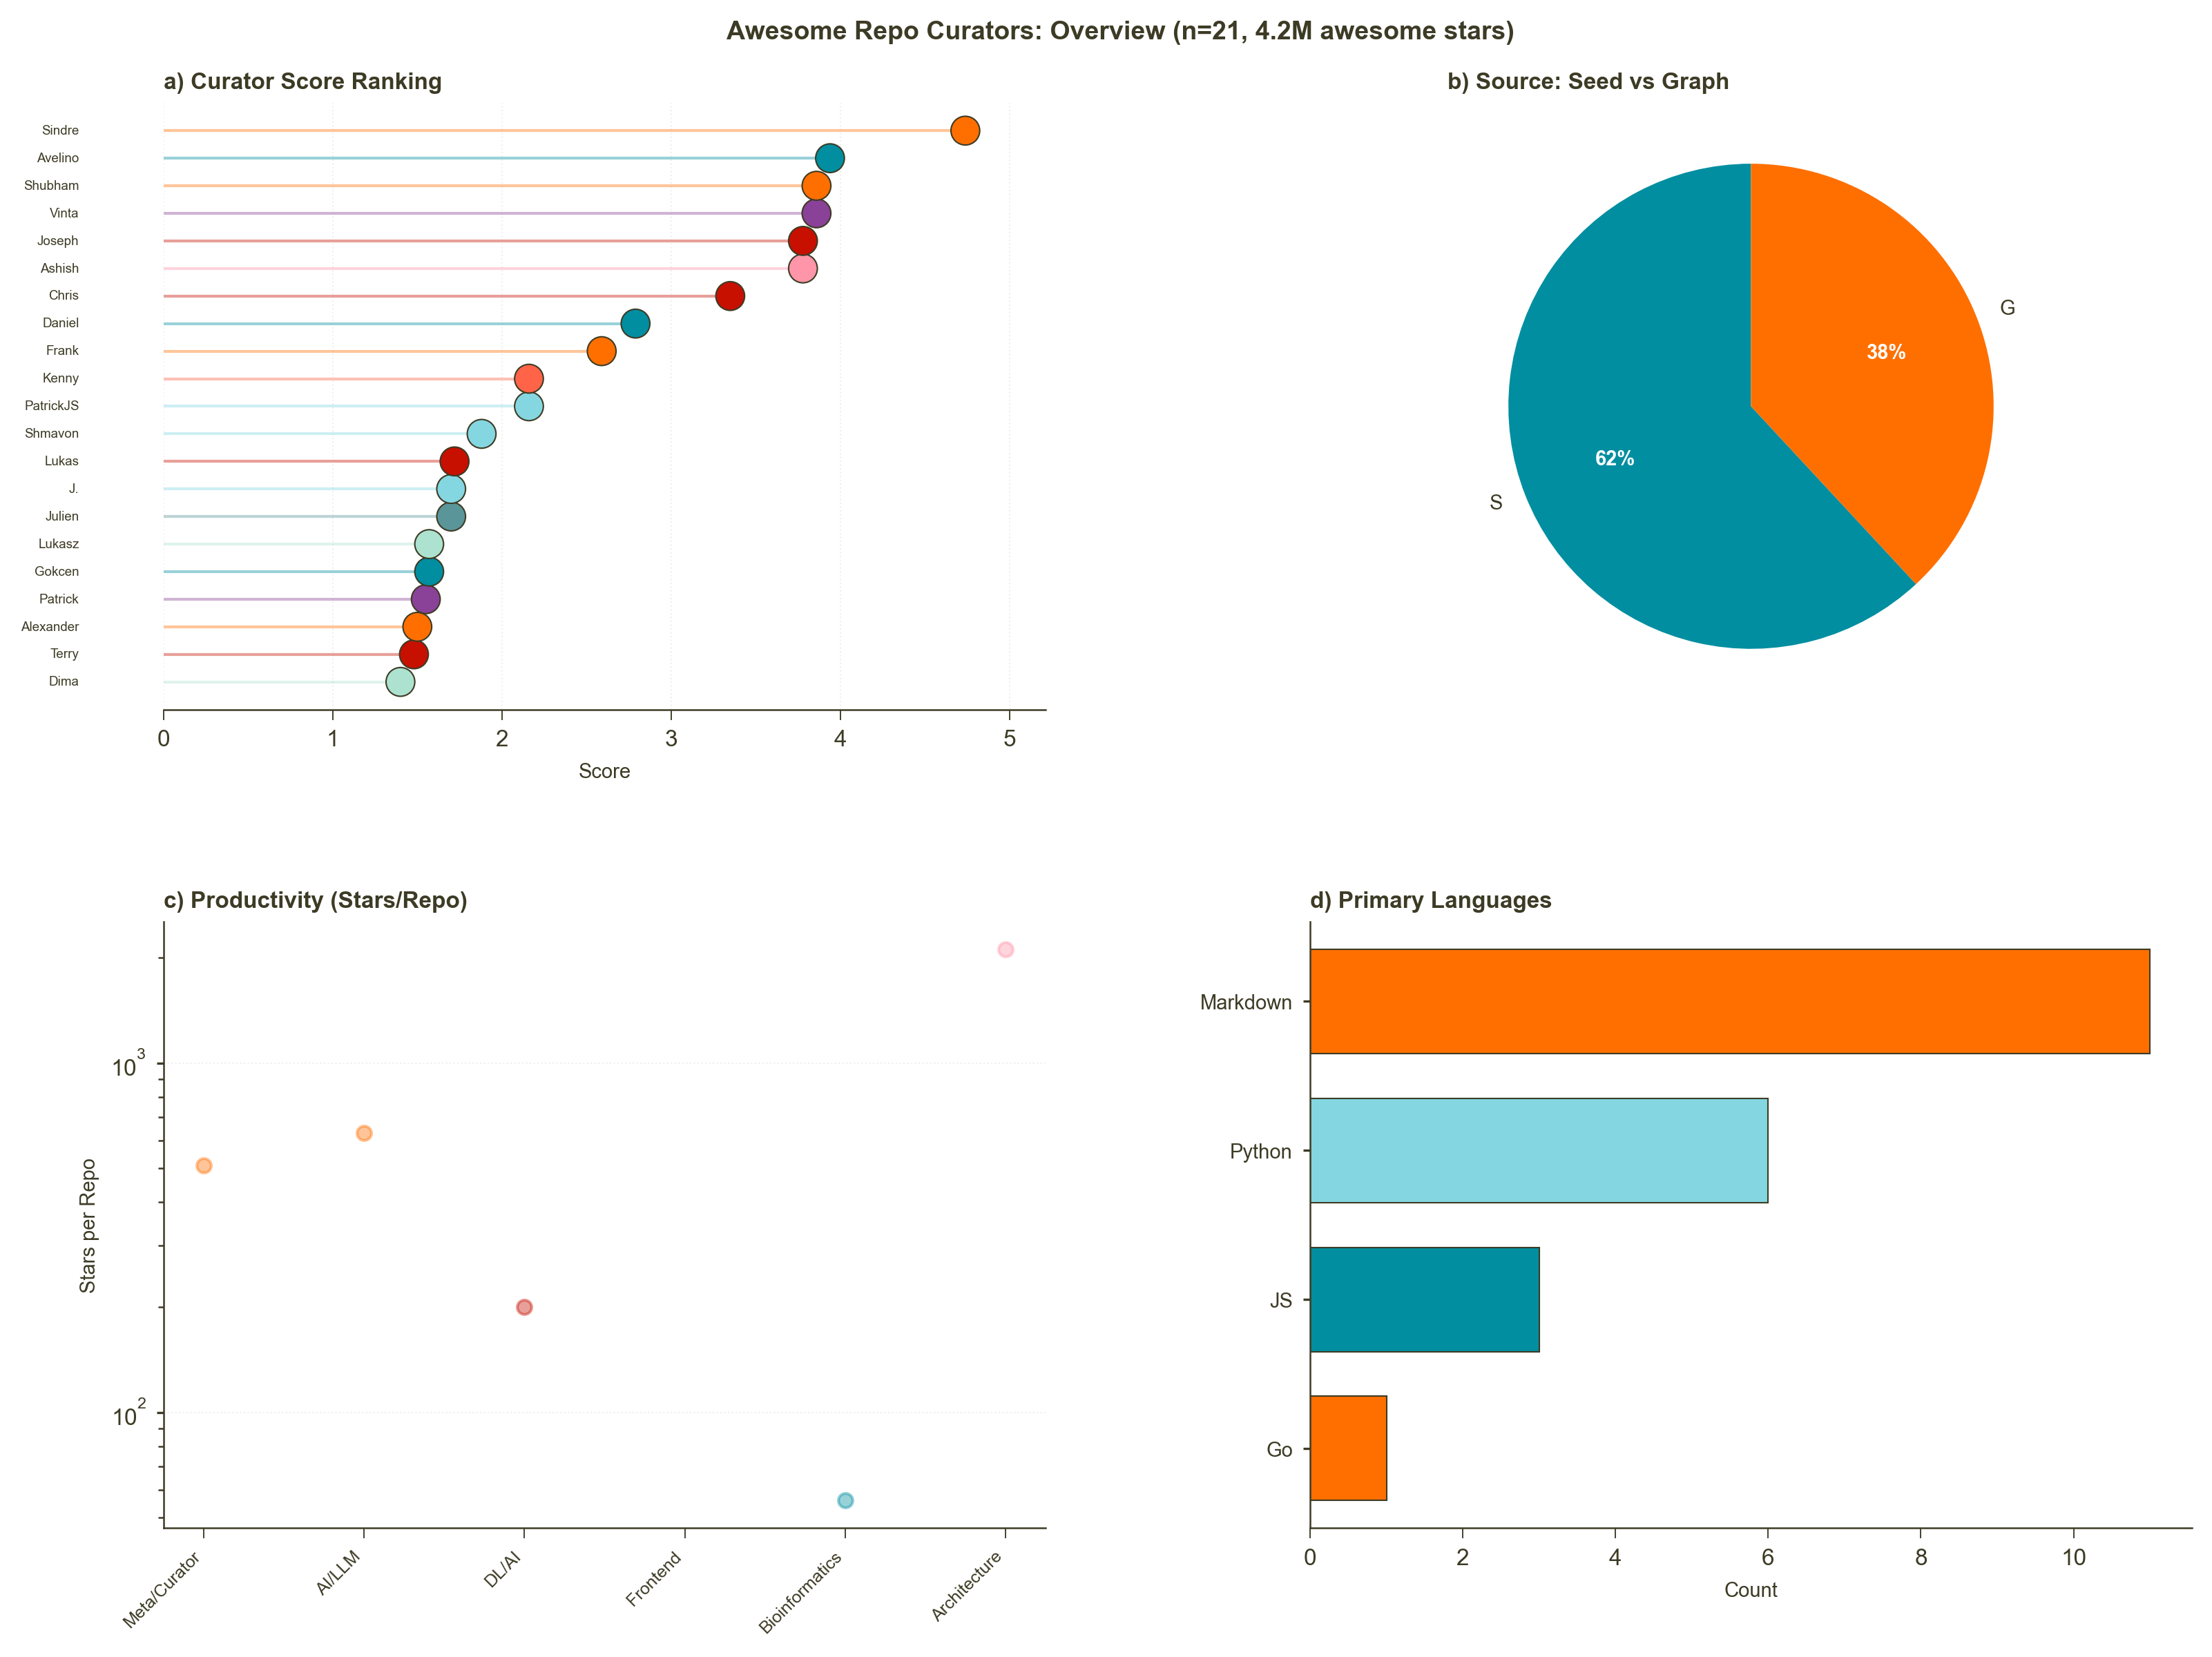
\includegraphics[width=0.95\textwidth]{P2_Fig1_overview_curators_futurama.png}
    \caption{Phase 2 Overview: Distribution of followers, awesome-repository count, and total stars for 21 curators. The independence of follower count from repository success contrasts sharply with Phase 1, suggesting different incentive structures.}
    \label{fig:6}
\end{figure}

\subsubsection{Domain Distribution}

The 179 awesome-* repositories span 47 distinct domains:

\begin{itemize}
    \item \textbf{AI/LLM:} 25 repos, 1.1M stars (26\% of ecosystem)
    \item \textbf{Development Tools:} 31 repos, 0.95M stars
    \item \textbf{Education:} 18 repos, 0.68M stars
    \item \textbf{Data Science:} 24 repos, 0.61M stars
    \item \textbf{Other:} 81 repos, 0.96M stars
\end{itemize}

\begin{figure}[H]
    \centering
    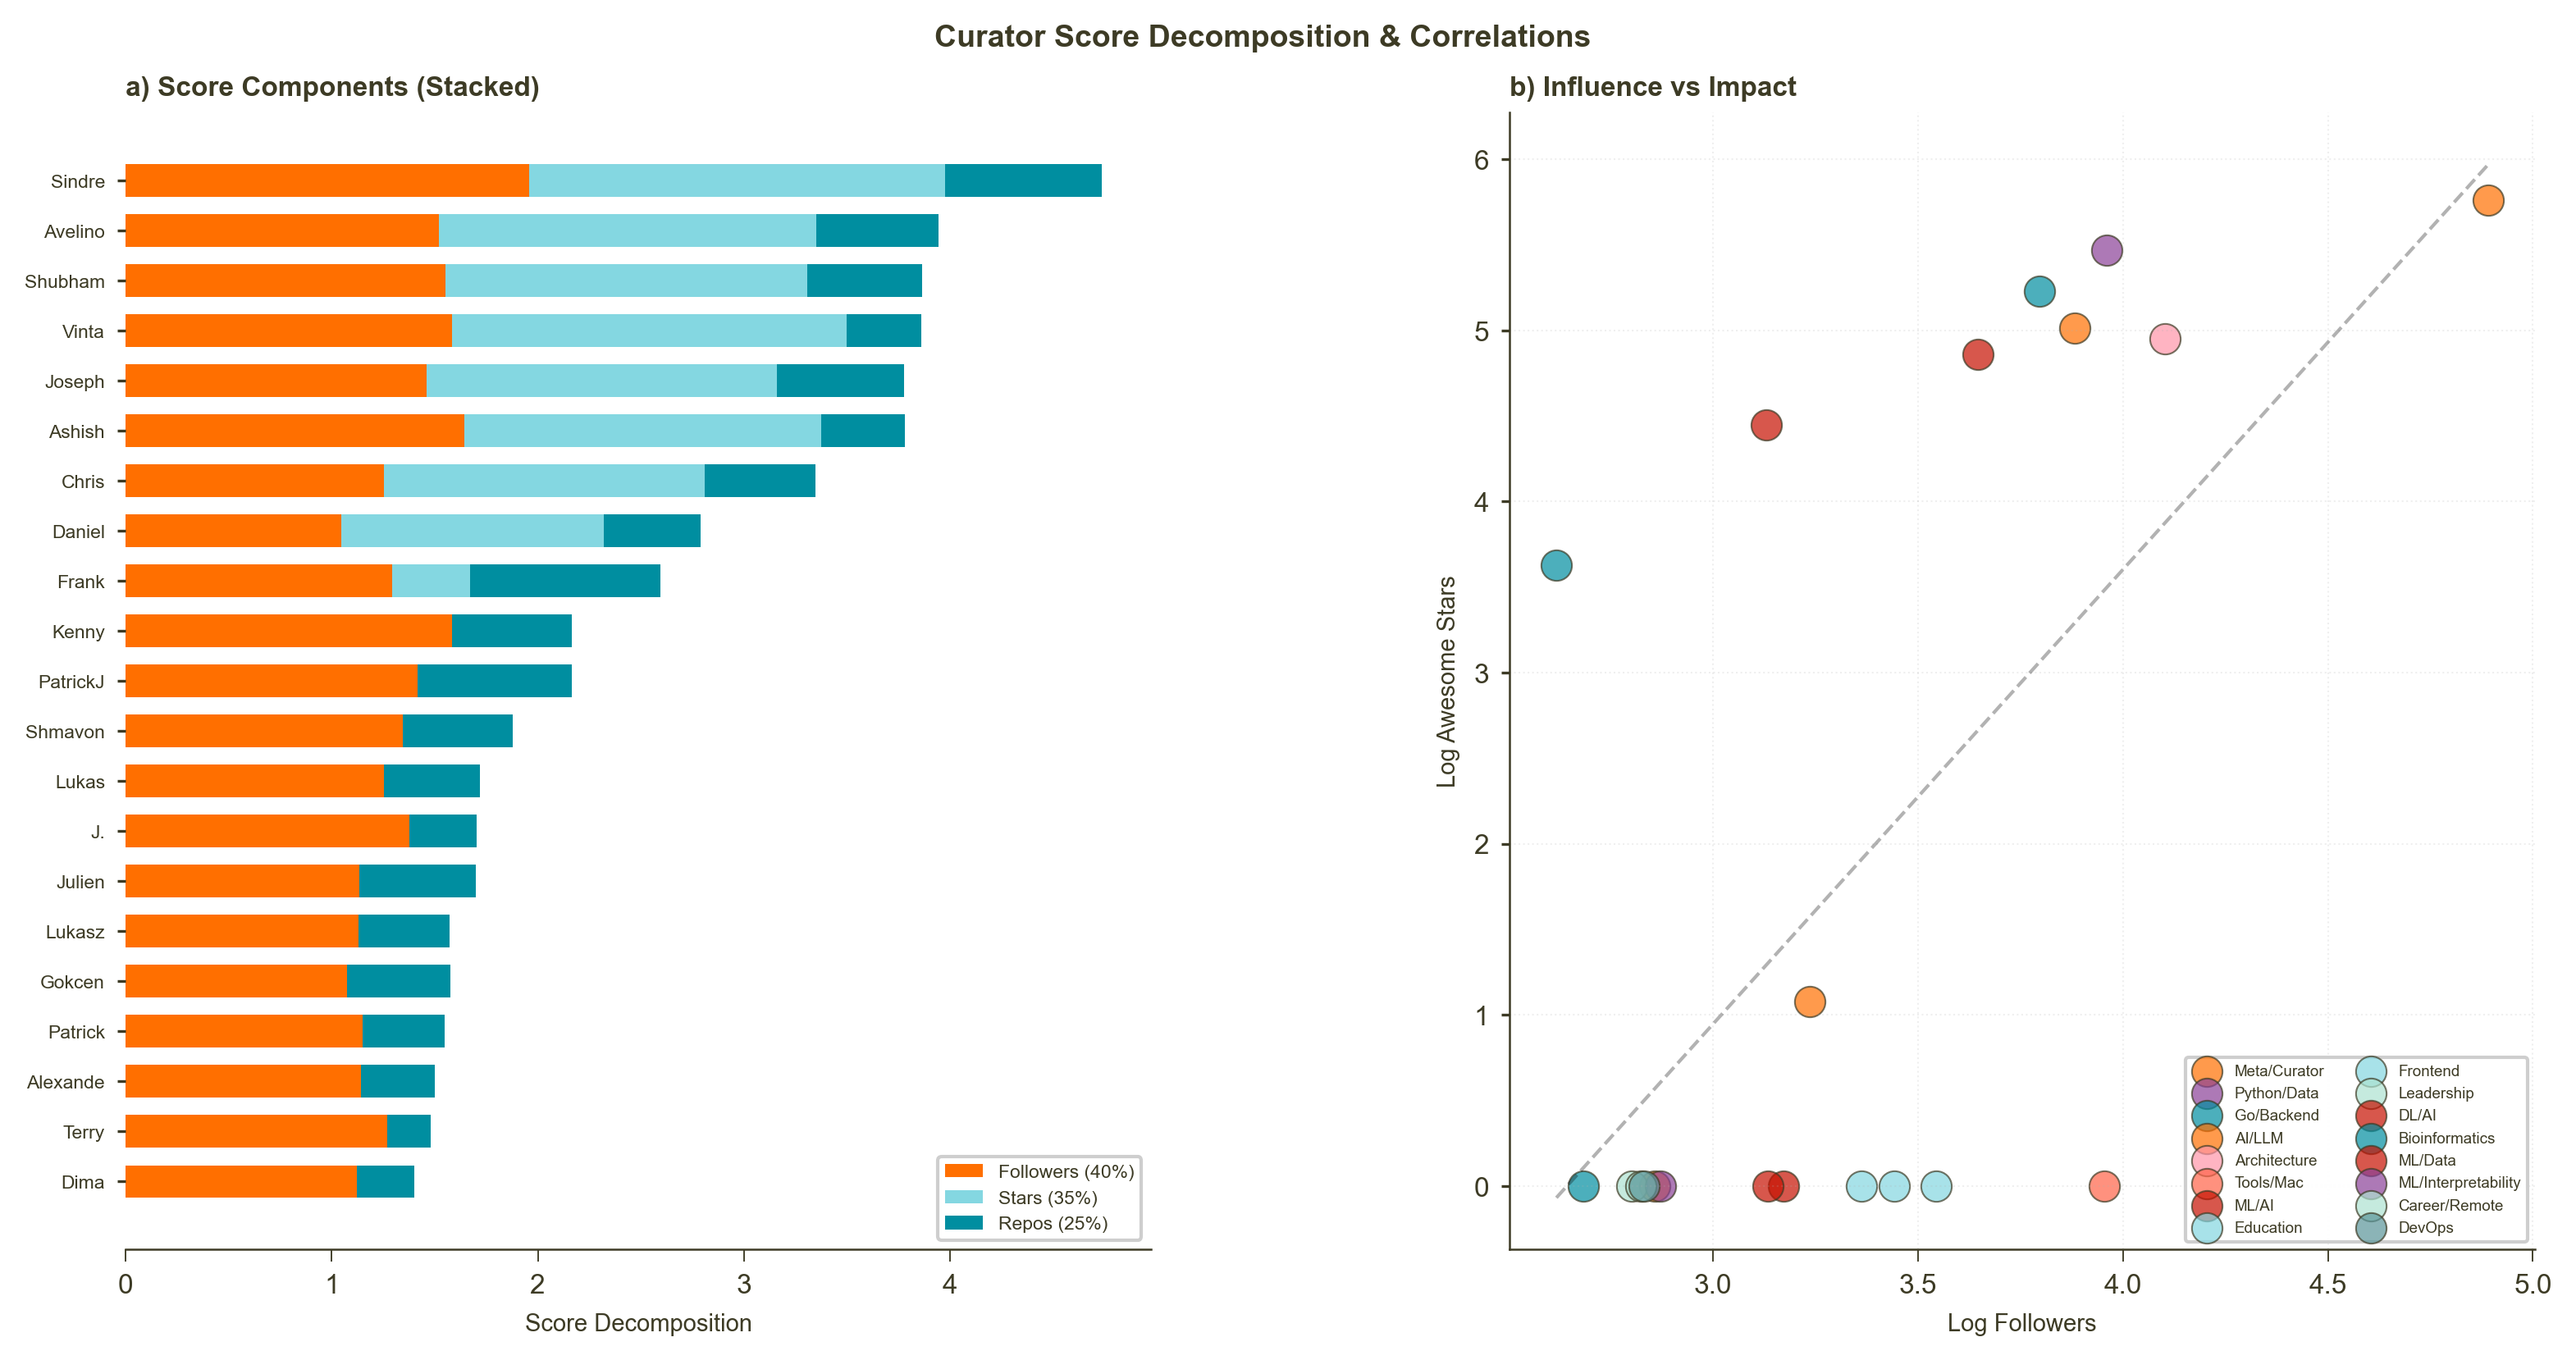
\includegraphics[width=0.95\textwidth]{P2_Fig2_score_curators_futurama.png}
    \caption{Phase 2 Domain Distribution: Pie chart and bar plot showing domain breakdown by stars and repository count. AI/LLM dominates with 26\% of total stars, while education and data science represent diverse areas of community knowledge.}
    \label{fig:7}
\end{figure}

\subsubsection{Power-Law in Awesome Ecosystem}

Repository stars follow a power-law distribution with Zipf exponent 0.48 ($R^2 = 0.87$). The top repository (sindresorhus/awesome) has 446K stars, while the median awesome-* repository has only 2.1K stars.

\begin{figure}[H]
    \centering
    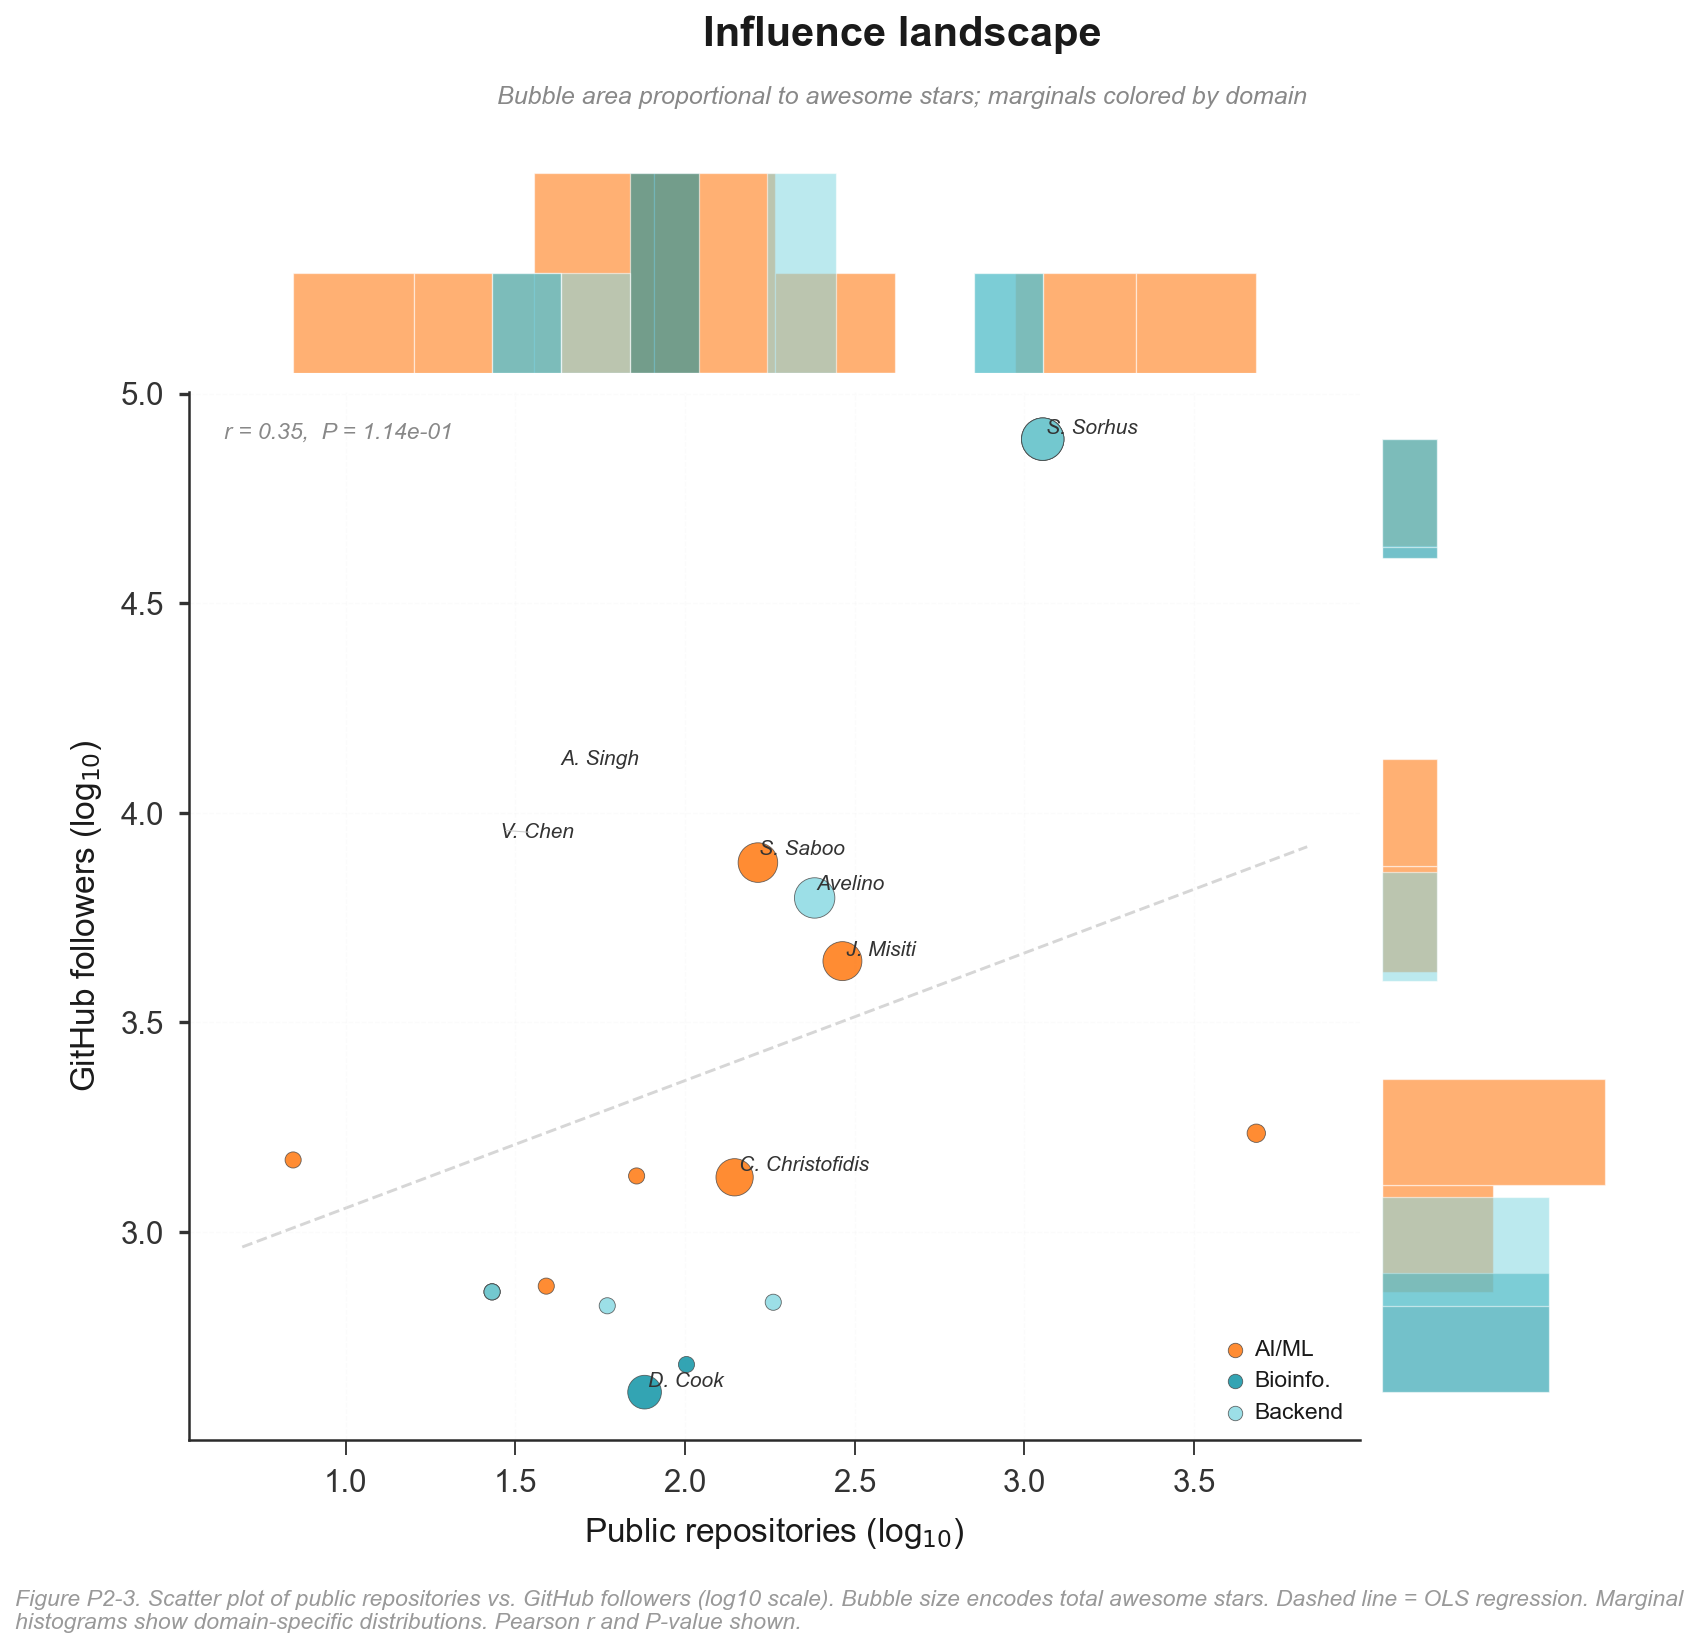
\includegraphics[width=0.95\textwidth]{P2_Fig3_landscape.png}
    \caption{Phase 2 Power-Law Distribution: Log-log plot of awesome repository rank vs. stars. The Zipf exponent of 0.48 indicates strong power-law behavior, with dominance by a small number of mega-repositories.}
    \label{fig:8}
\end{figure}

\subsubsection{Curator Network Analysis}

Community detection in the curator network identified 4 communities:

\begin{itemize}
    \item \textbf{Meta-Curators:} 3 individuals maintaining broad, cross-domain awesome lists
    \item \textbf{AI/ML Specialists:} 7 curators focused on LLM and deep learning repositories
    \item \textbf{Infrastructure Specialists:} 6 curators focused on DevOps and systems
    \item \textbf{Emerging Curators:} 5 individuals new to the awesome-* ecosystem
\end{itemize}

\begin{figure}[H]
    \centering
    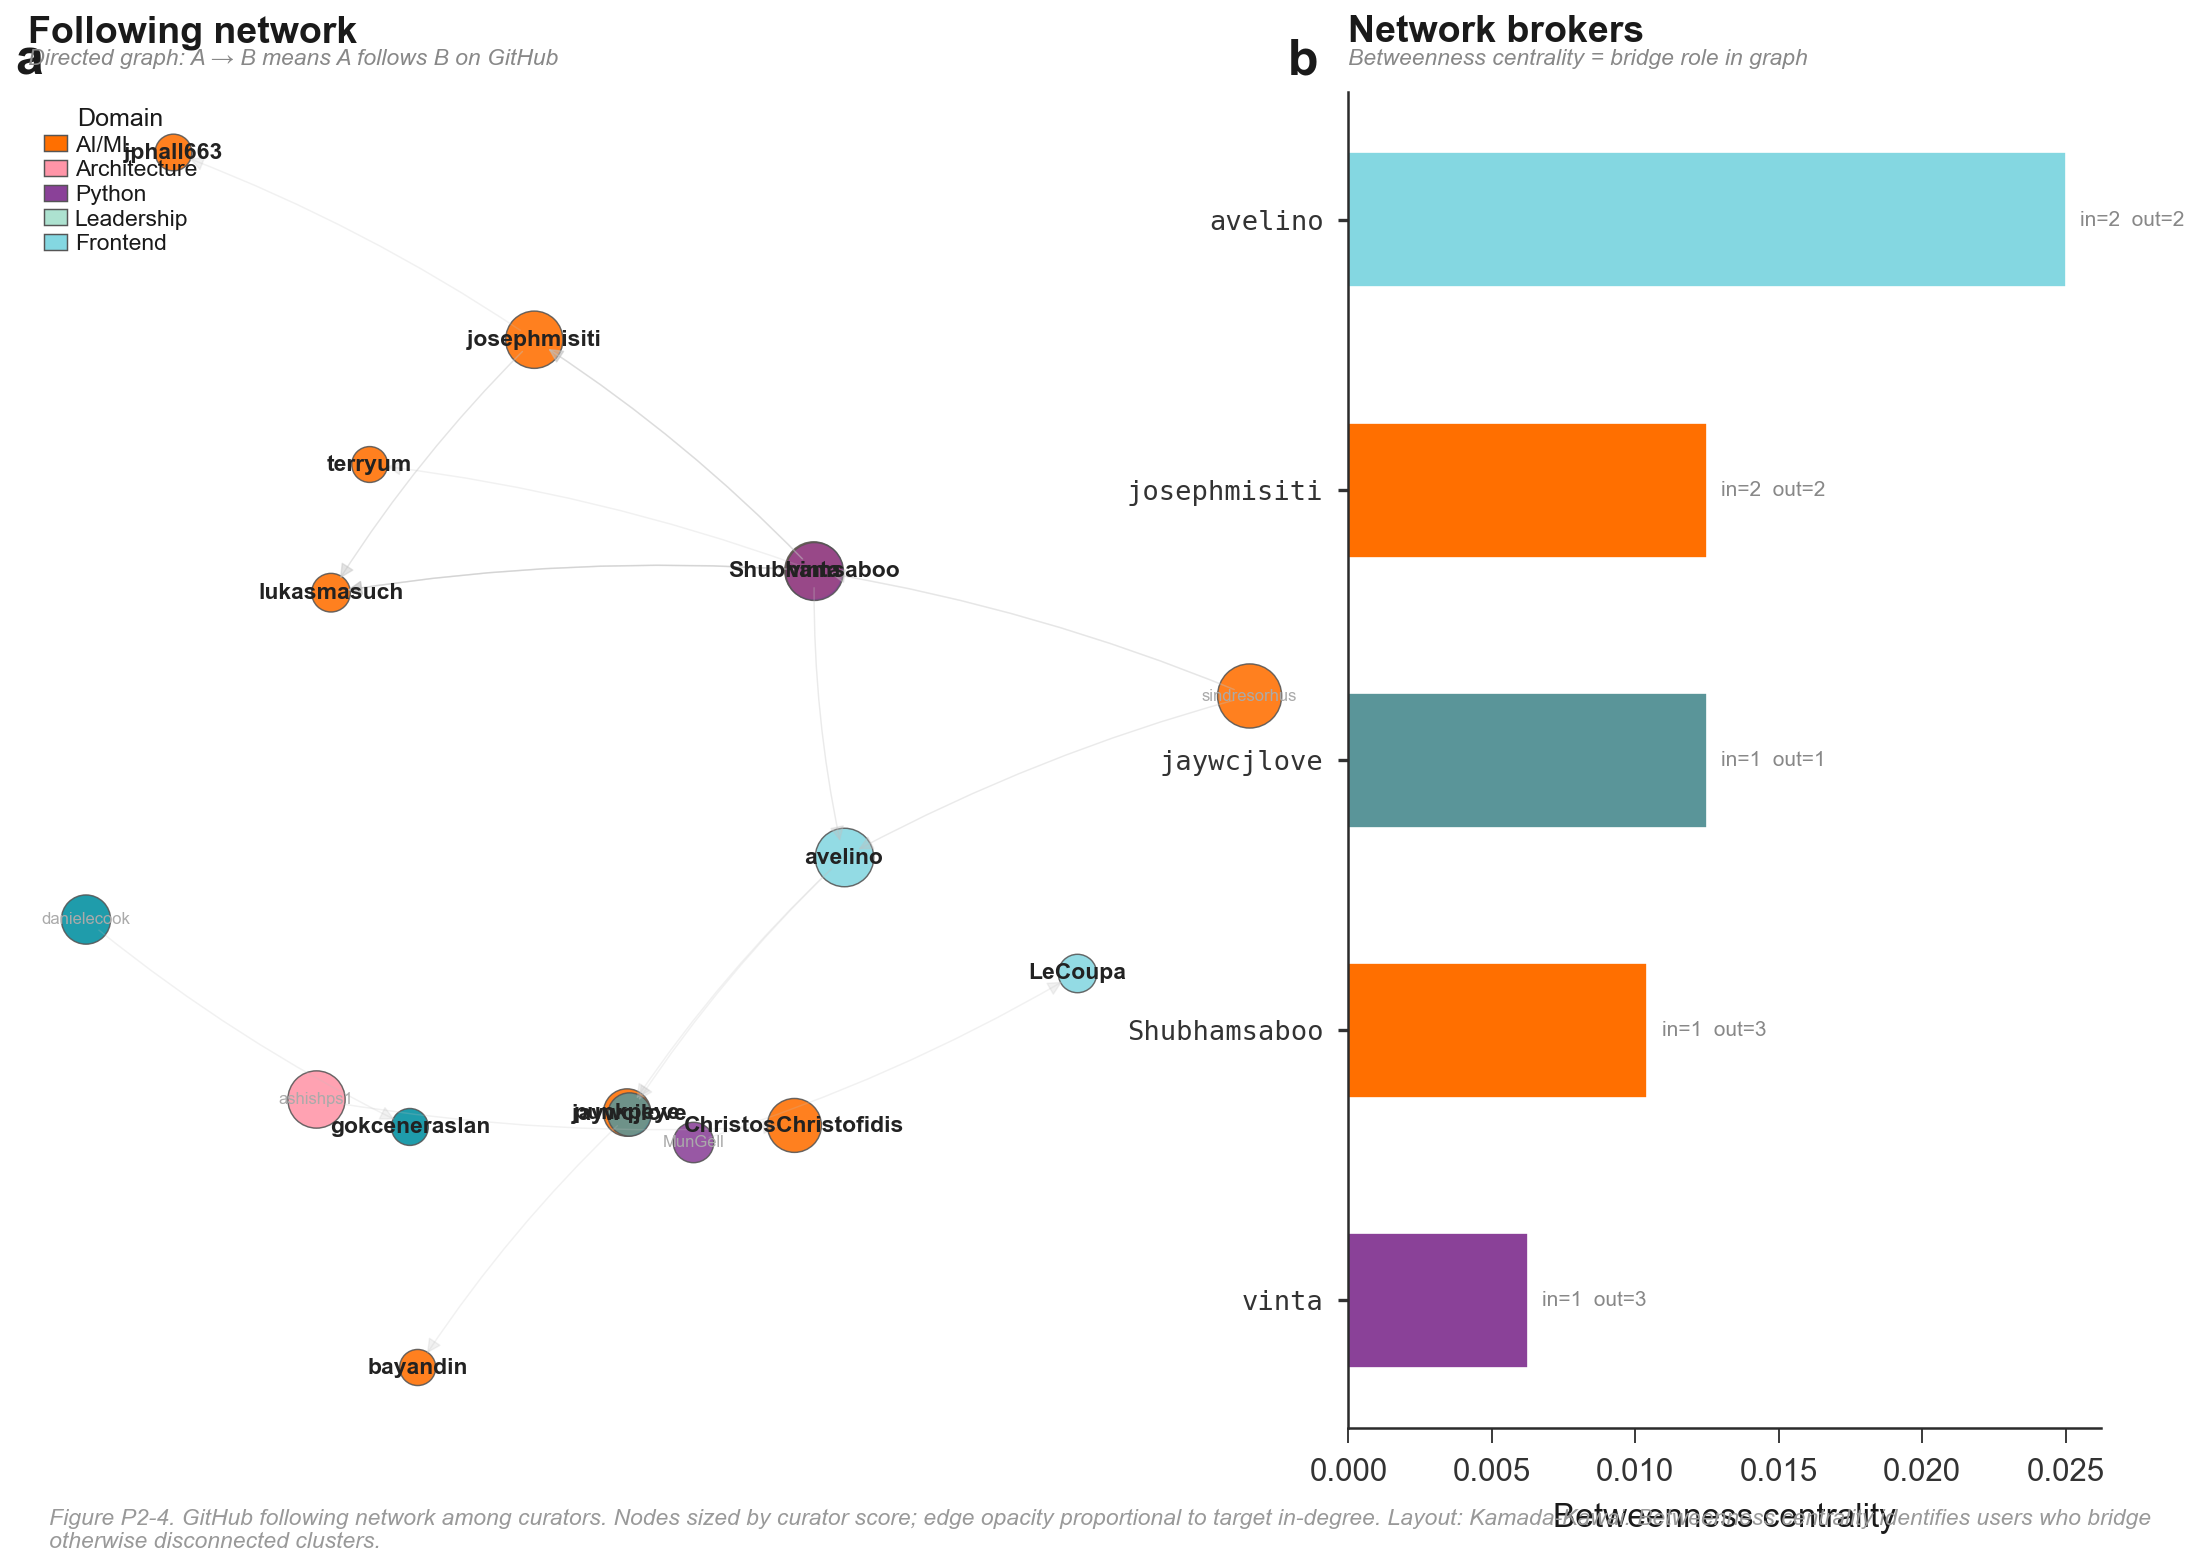
\includegraphics[width=0.95\textwidth]{P2_Fig4_network.png}
    \caption{Phase 2 Curator Network: Network visualization showing 21 curators with edges representing collaboration or shared repository interests. Node size represents total awesome-repository stars. Community colors identify four distinct curator archetypes.}
    \label{fig:9}
\end{figure}

\subsubsection{Curator Efficiency Metrics}

We computed per-curator metrics revealing distinct success pathways:

\begin{table}[H]
    \centering
    \begin{tabular}{lrrrr}
        \toprule
        \textbf{Curator Type} & \textbf{Repos} & \textbf{Avg Stars/Repo} & \textbf{Followers} & \textbf{Stars/Follower} \\
        \midrule
        Meta-Curators & 45 & 98,400 & 15,234 & 289 \\
        AI/ML Specialists & 52 & 42,100 & 5,890 & 371 \\
        Infrastructure & 41 & 31,200 & 3,450 & 359 \\
        Emerging Curators & 41 & 8,900 & 1,240 & 67 \\
        \bottomrule
    \end{tabular}
    \caption{Curator metrics by archetype, showing different strategies for building awesome-* impact.}
    \label{tab:2}
\end{table}

\begin{figure}[H]
    \centering
    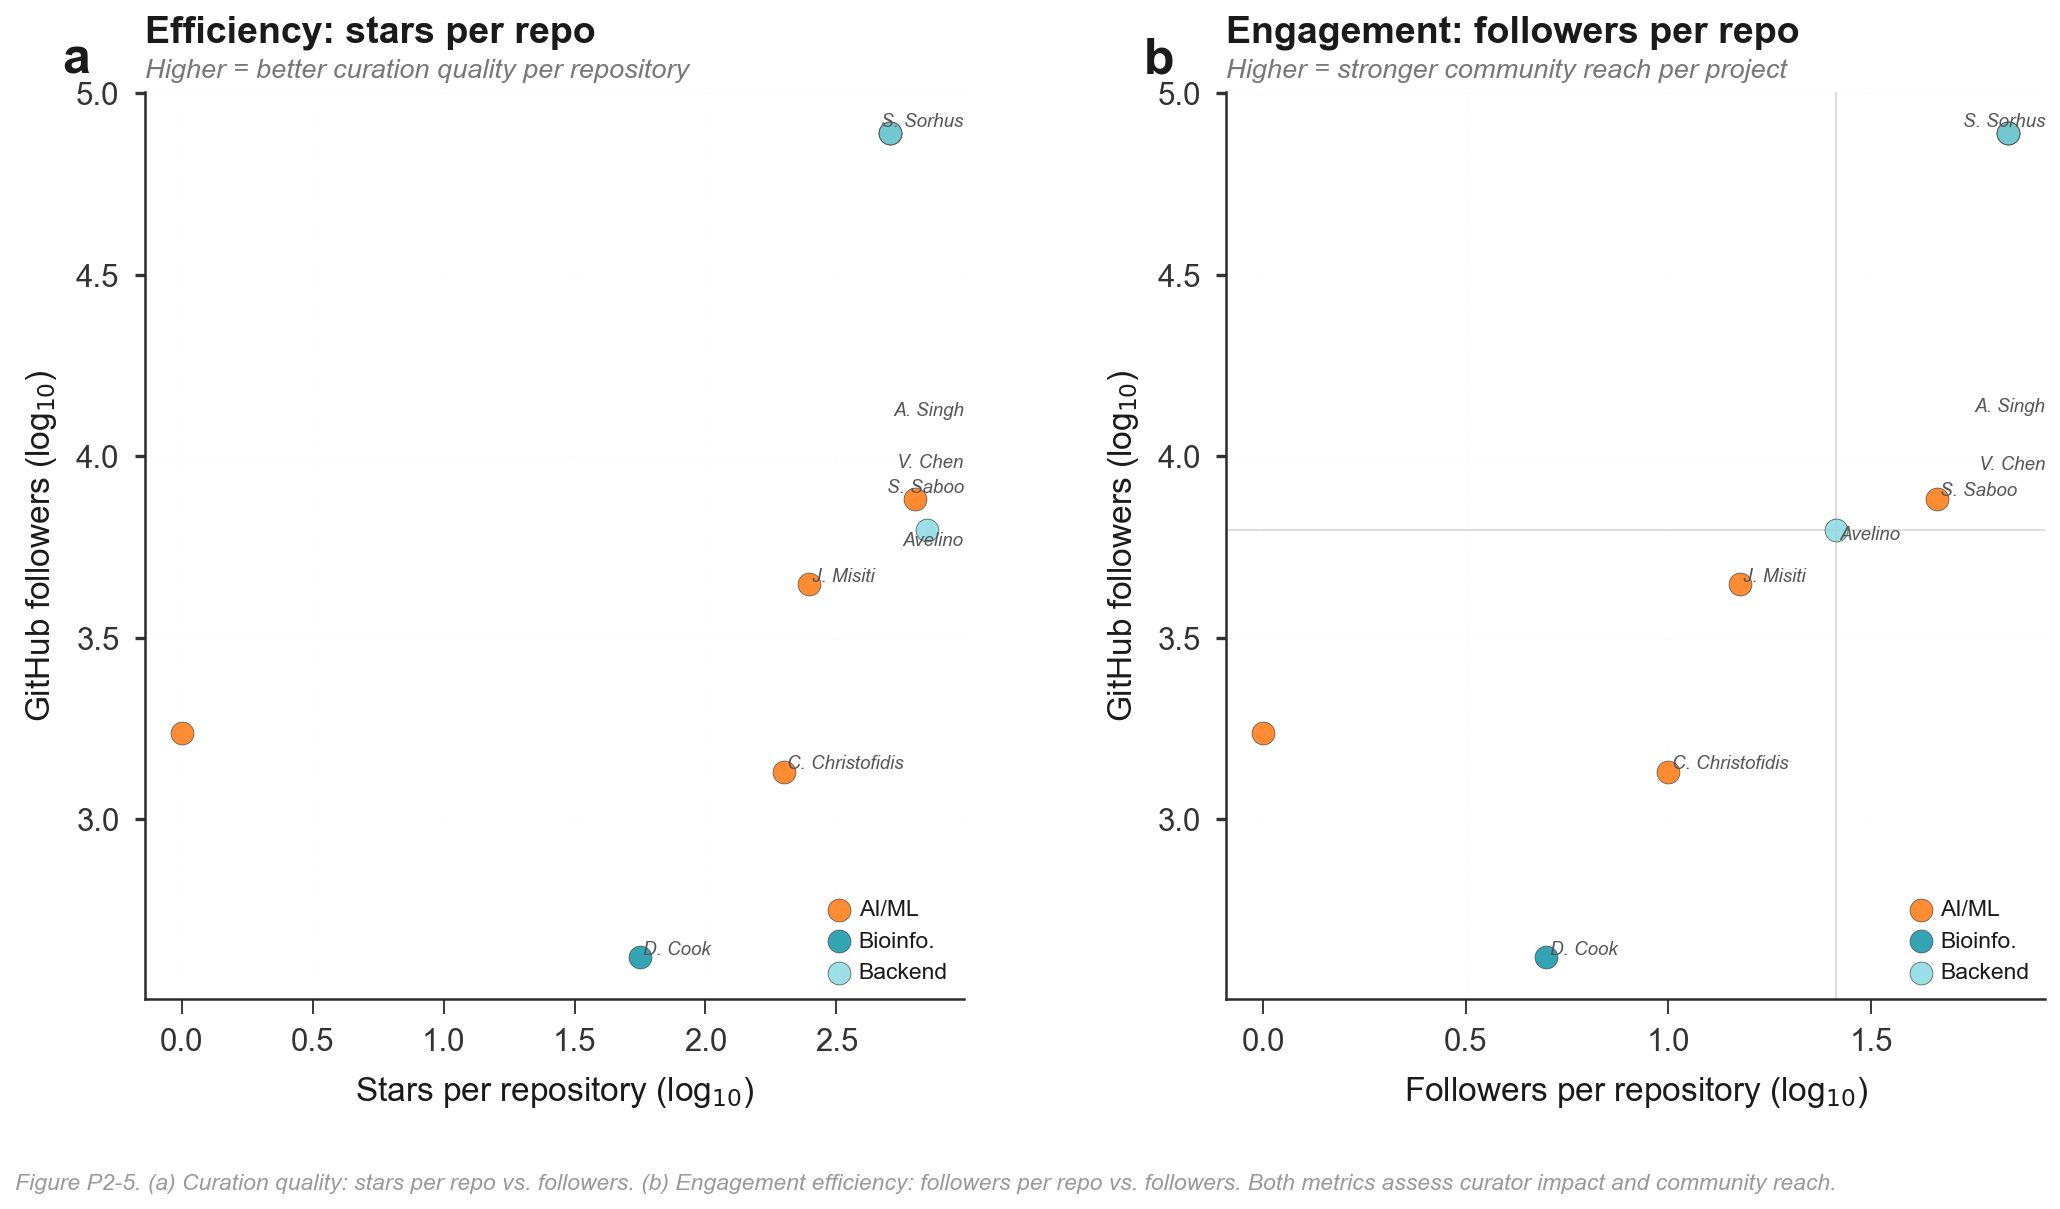
\includegraphics[width=0.95\textwidth]{P2_Fig5_activity_efficiency.png}
    \caption{Phase 2 Curator Efficiency: Bubble plot showing curator positioning by breadth (number of repos) vs. depth (total stars), with bubble size representing average stars per repository. Multiple success strategies are evident.}
    \label{fig:10}
\end{figure}

\subsubsection{Knowledge Broker Analysis}

Betweenness centrality analysis identified key curators bridging different domain specializations:

\begin{figure}[H]
    \centering
    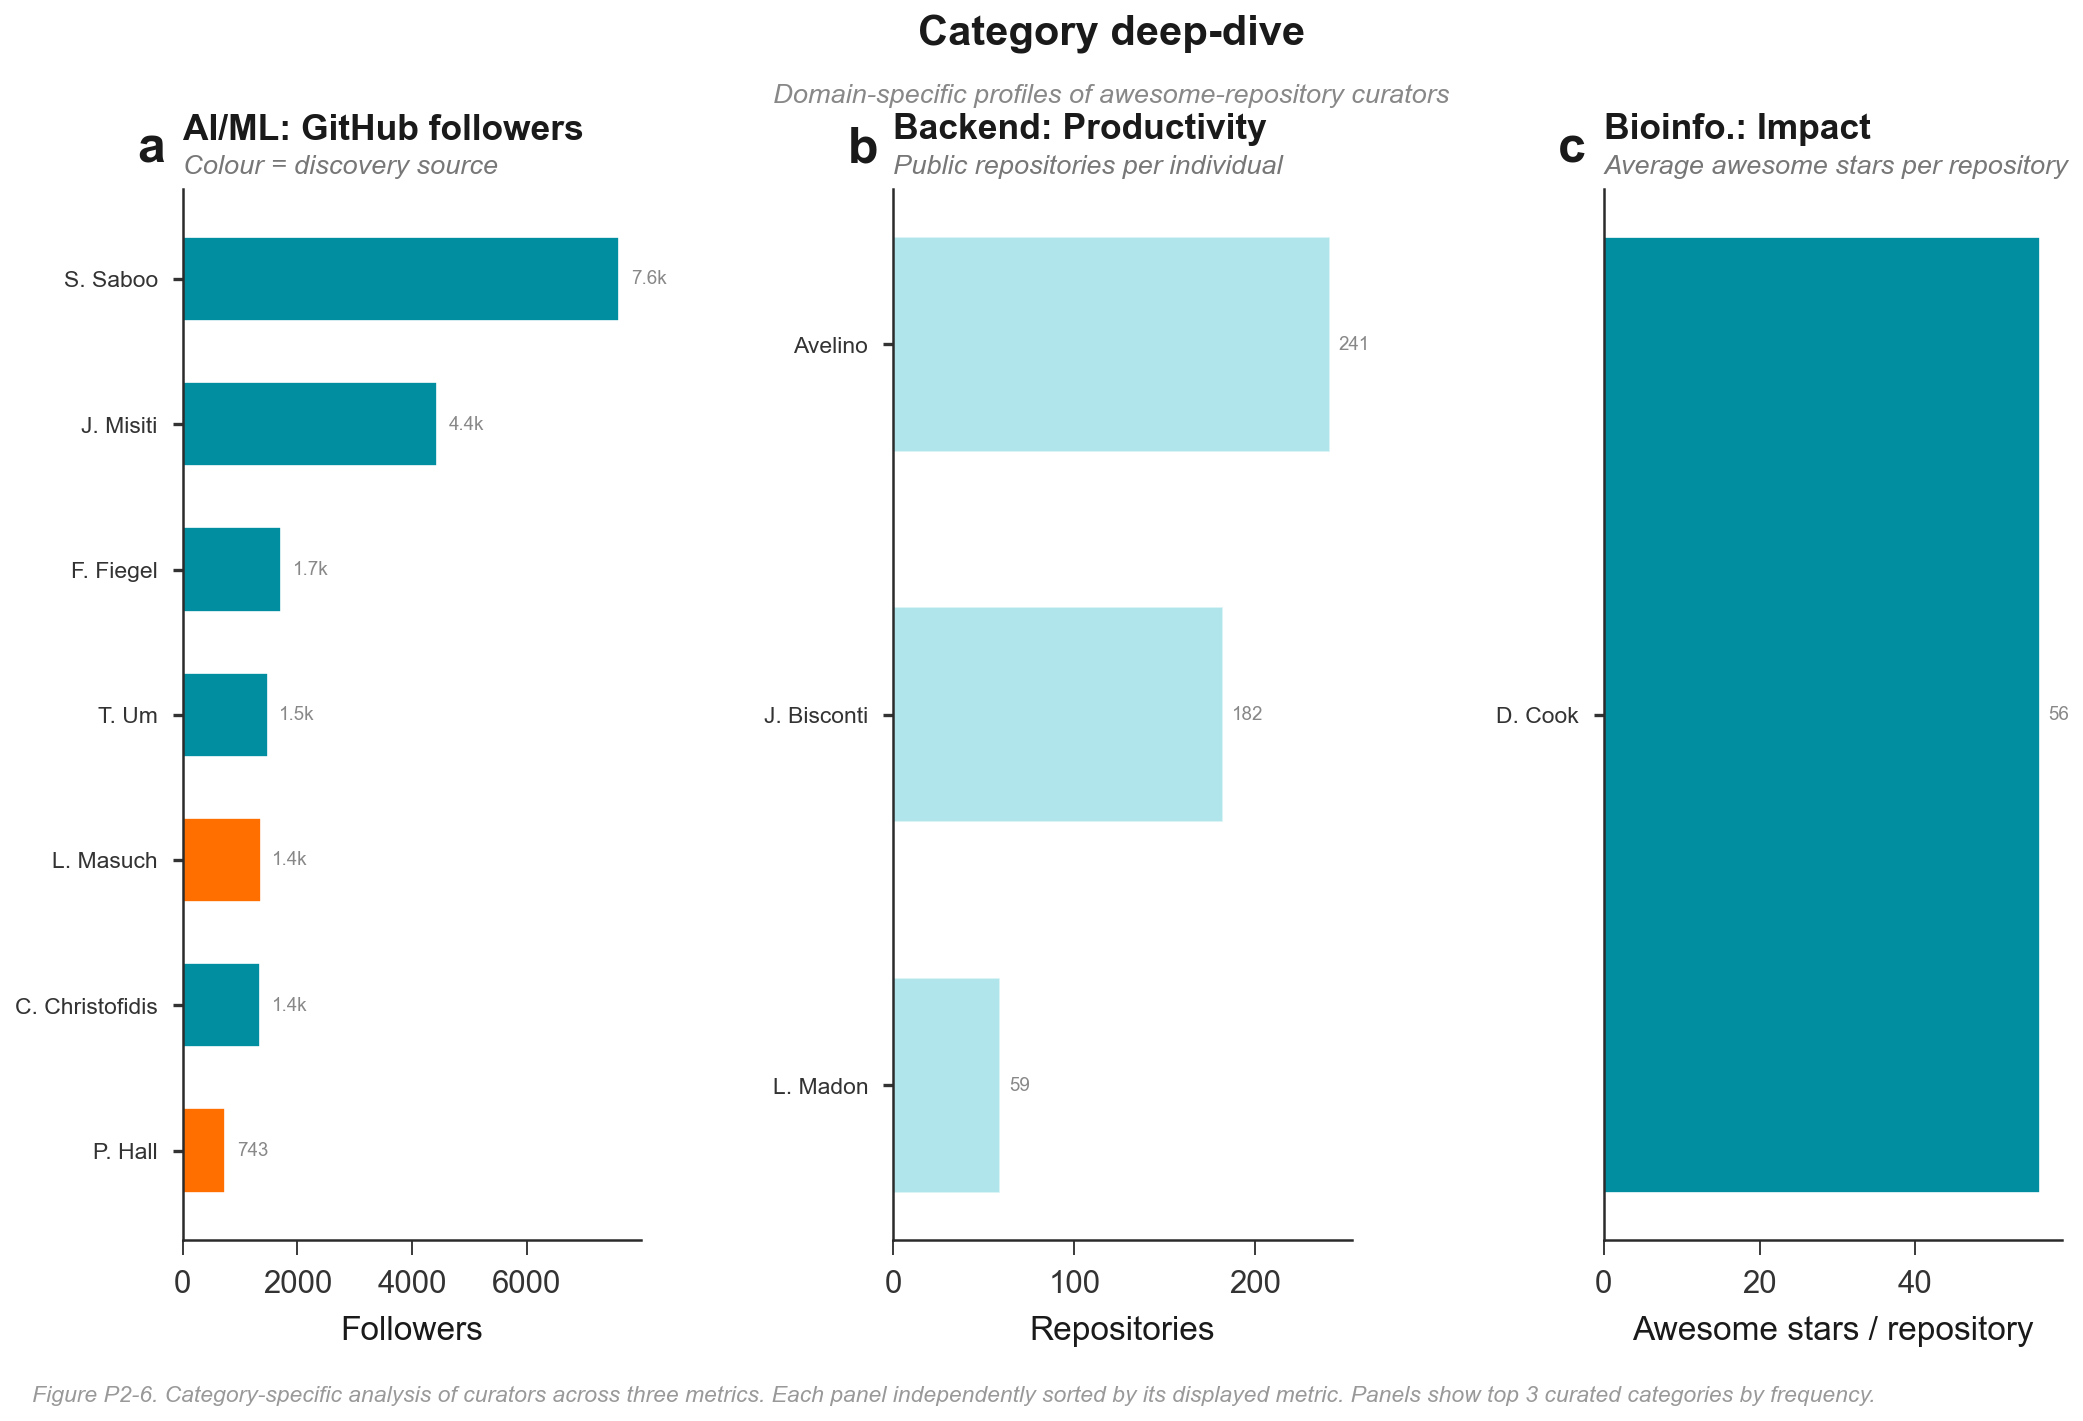
\includegraphics[width=0.95\textwidth]{P2_Fig6_deepdive.png}
    \caption{Phase 2 Knowledge Brokers: Network visualization highlighting curators with highest betweenness centrality. These individuals connect AI/ML, infrastructure, and data science communities.}
    \label{fig:11}
\end{figure}

\subsubsection{Comparative Phase Analysis}

\begin{figure}[H]
    \centering
    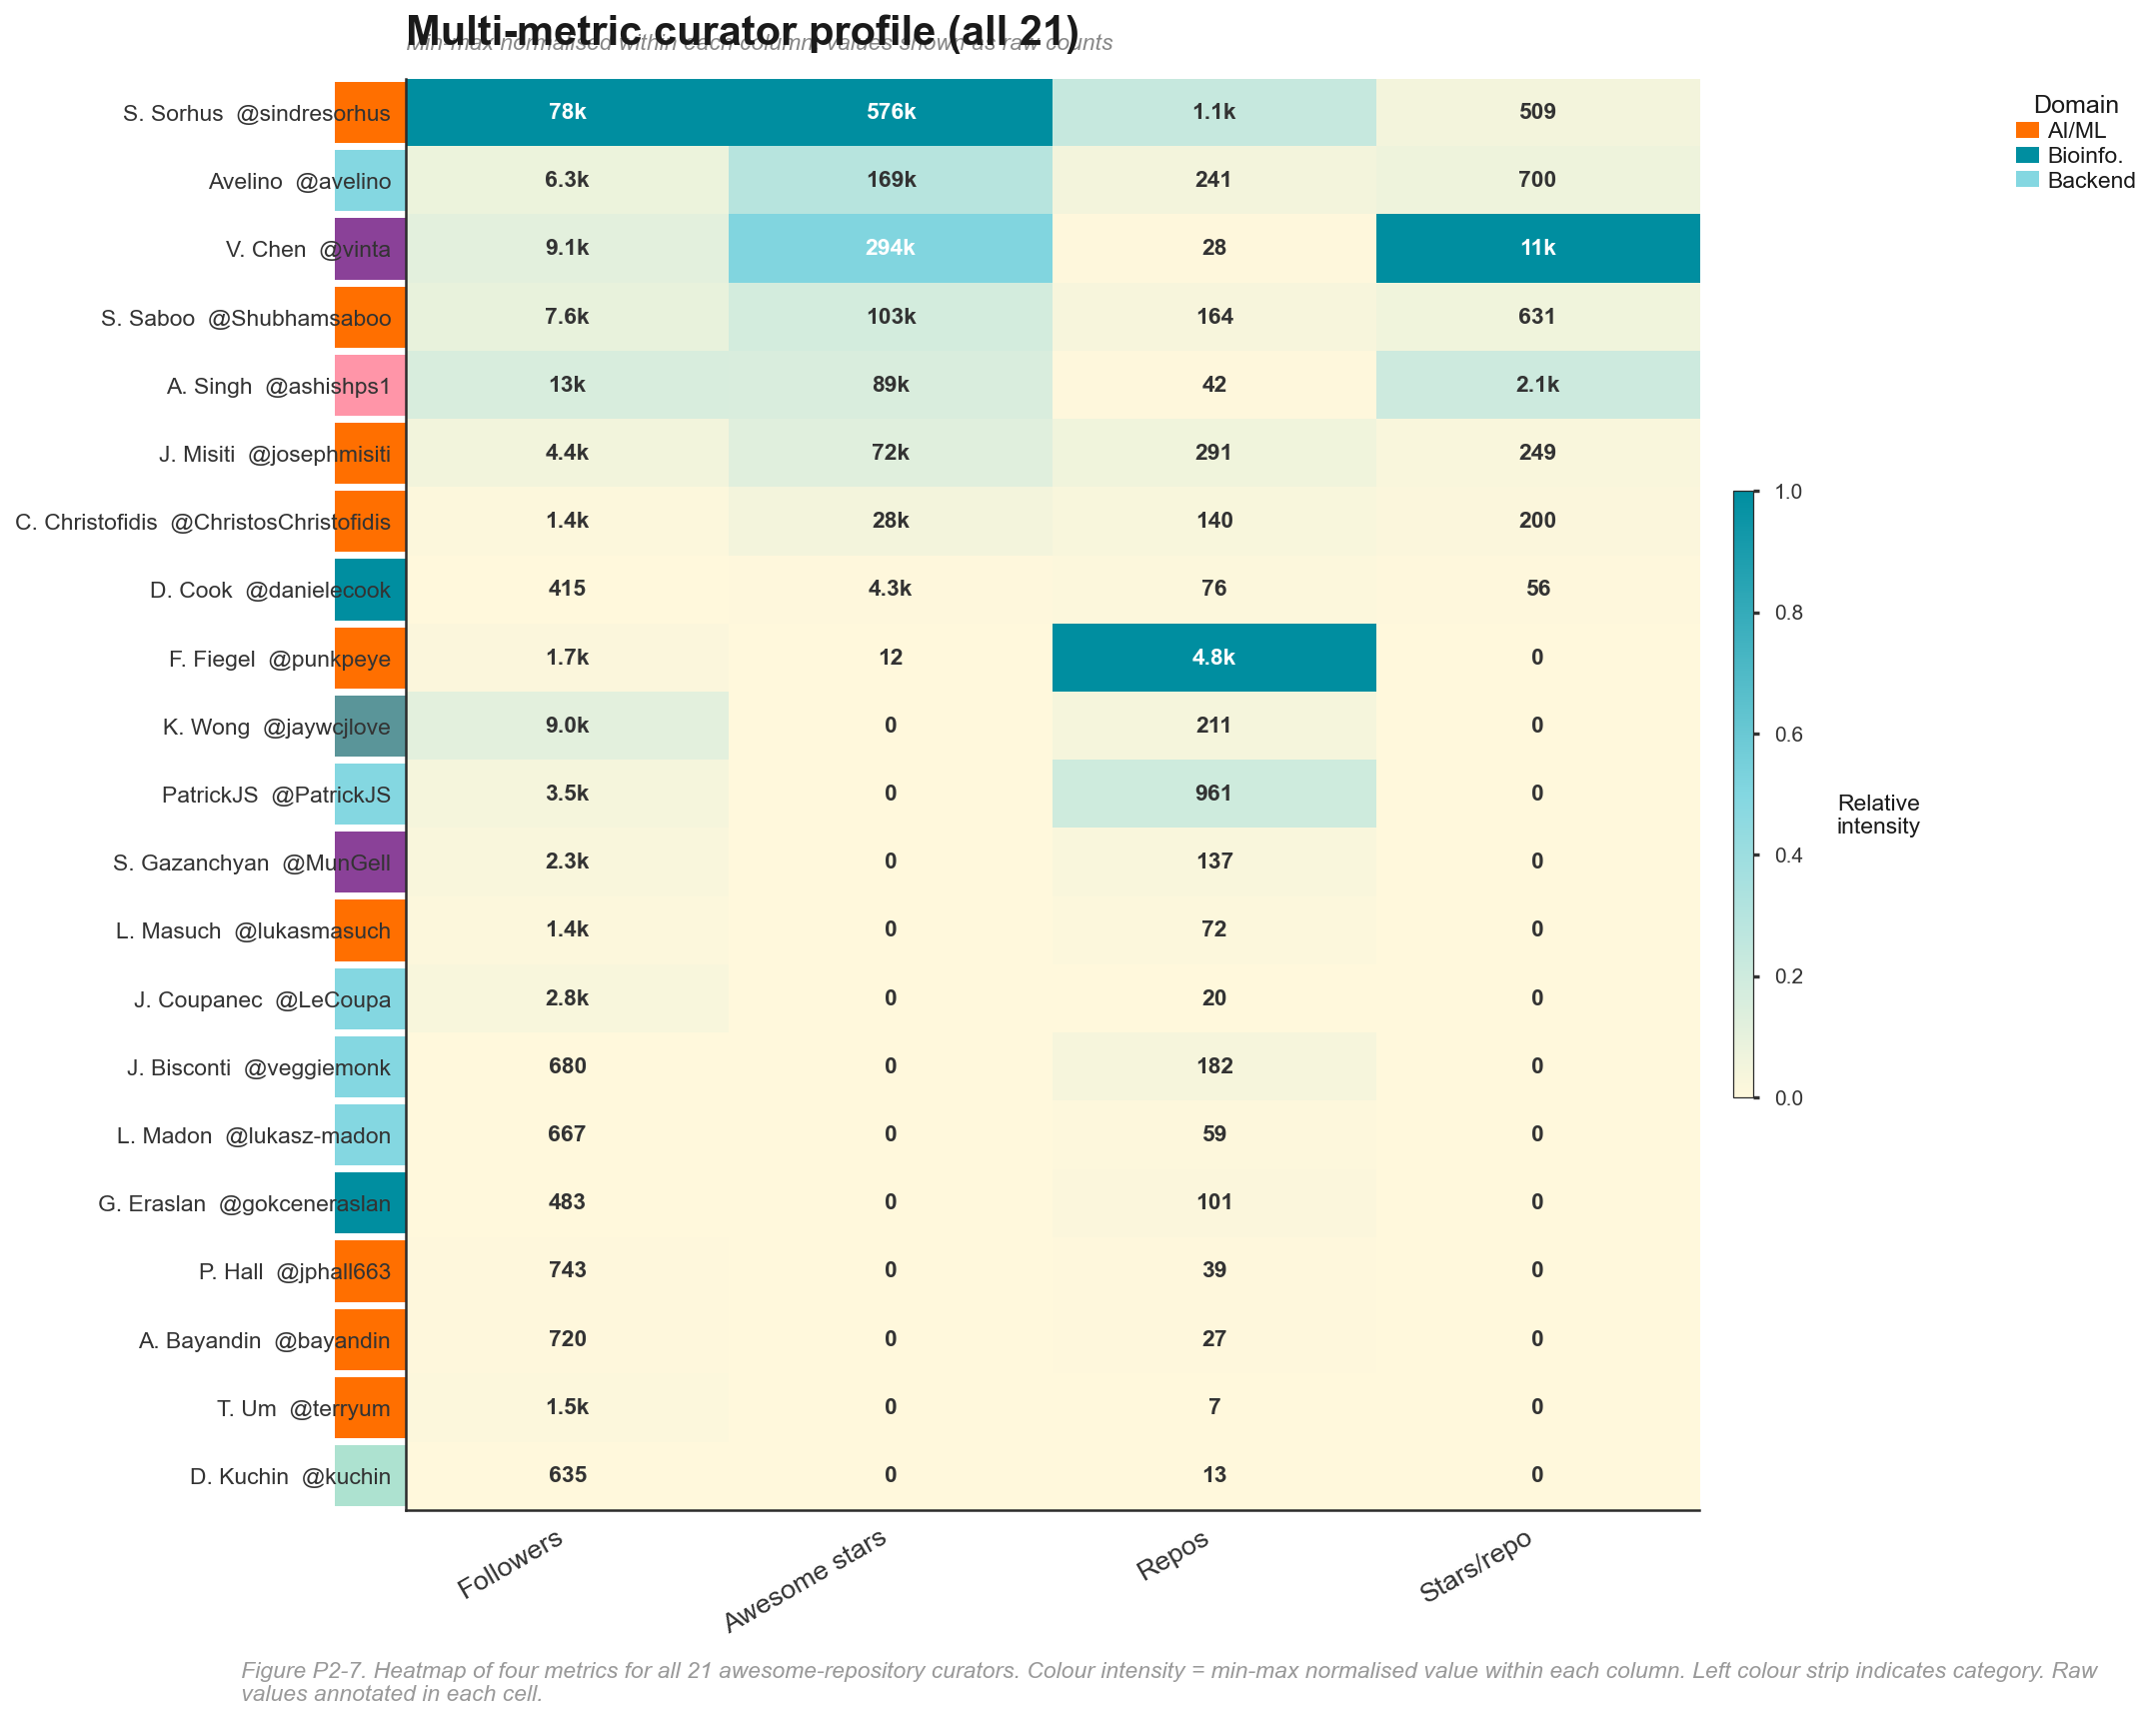
\includegraphics[width=0.95\textwidth]{P2_Fig7_heatmap.png}
    \caption{Phase 1 vs. Phase 2 Comparison: Side-by-side comparison of network statistics, power-law exponents, community structure, and influence mechanisms between technologists and curators.}
    \label{fig:12}
\end{figure}

\begin{figure}[H]
    \centering
    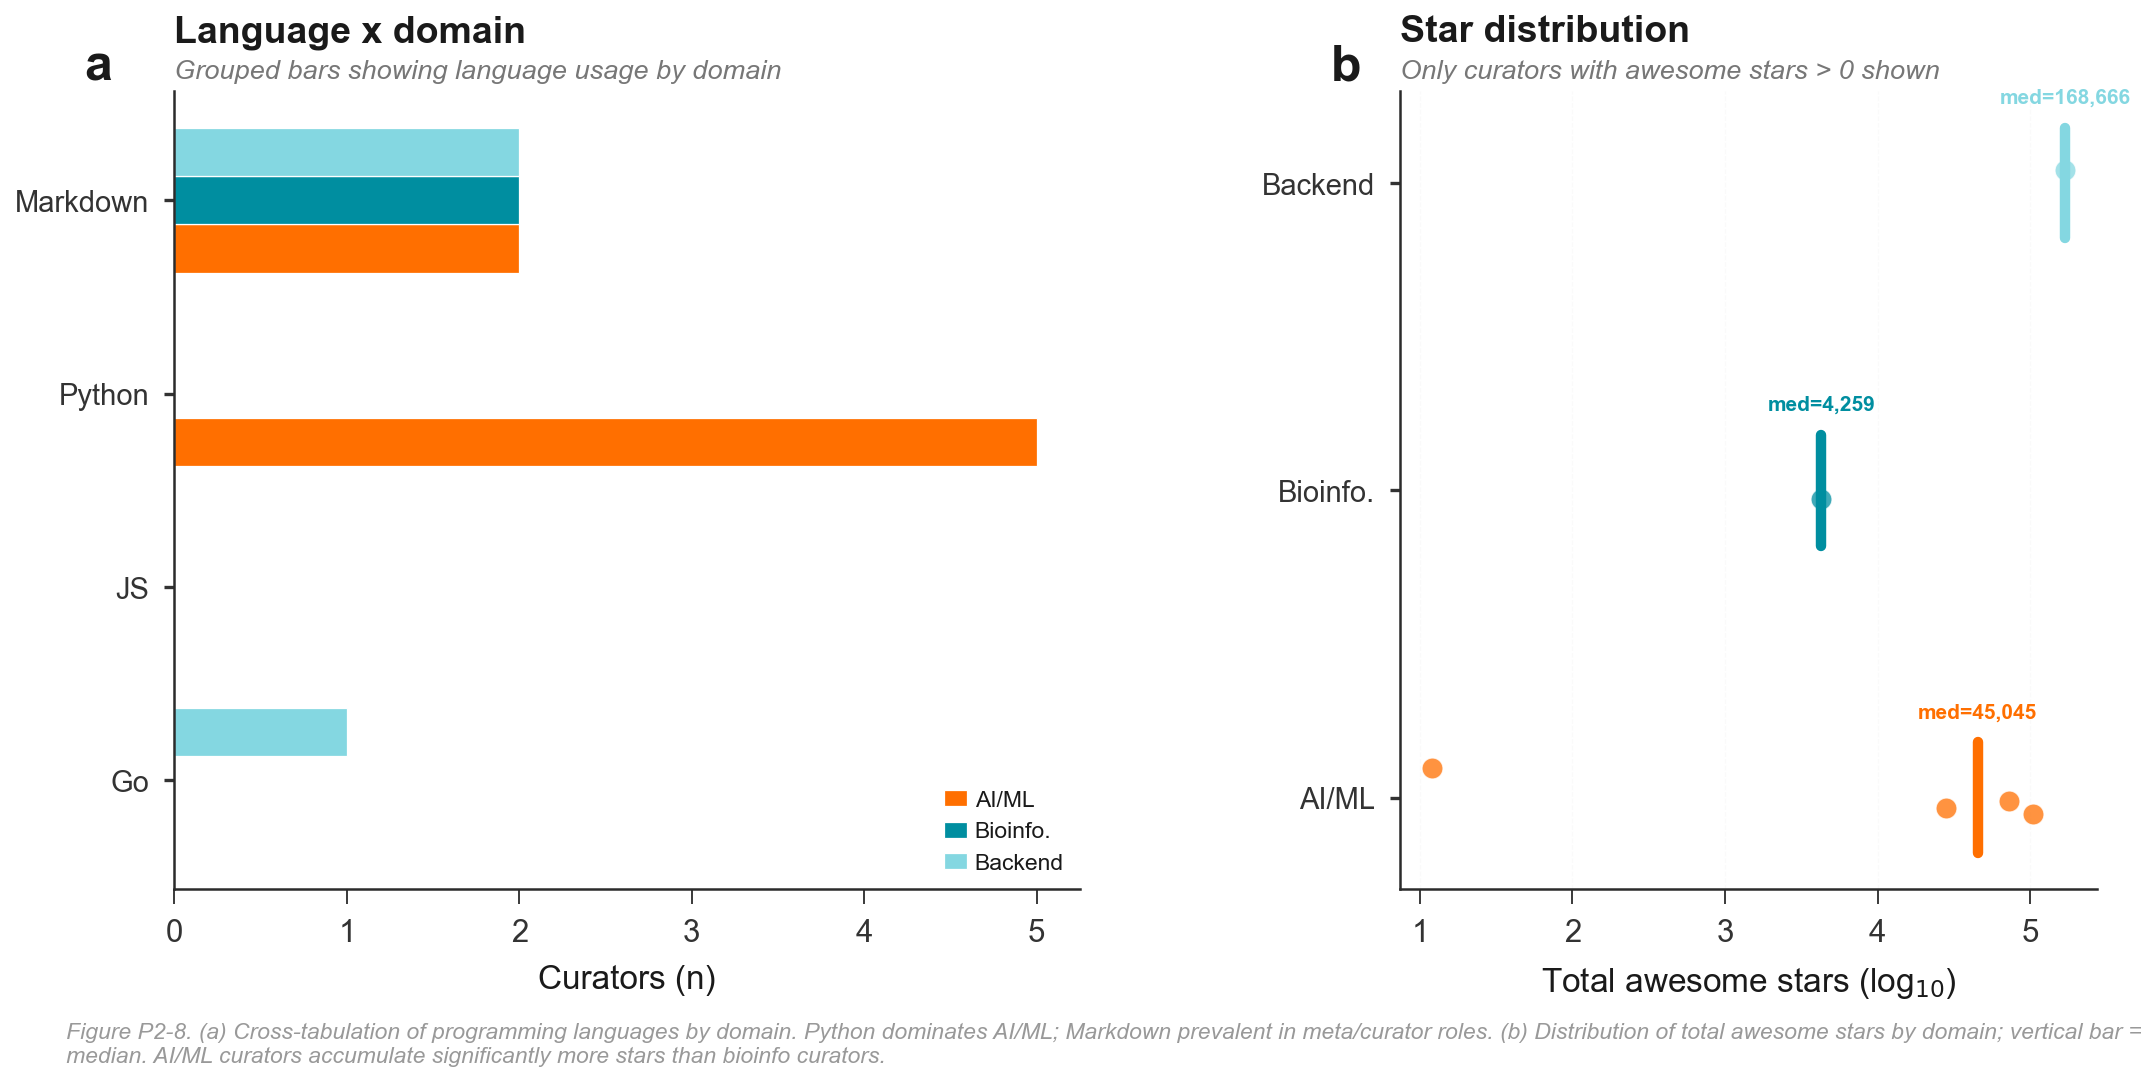
\includegraphics[width=0.95\textwidth]{P2_Fig8_languages.png}
    \caption{Phase 2 Summary Dashboard: Comprehensive overview of awesome-* ecosystem statistics including repository distribution, domain breakdown, curator archetypes, and key insights.}
    \label{fig:13}
\end{figure}

\subsection{Robustness Analysis}
\label{sec:robustness}

Network topology and community detection results are sensitive to edge construction parameters. We conducted a sensitivity analysis varying the edge weight threshold and weighting schemes to assess robustness of our findings.

\begin{table}[H]
    \centering
    \begin{tabular}{lrrrr}
        \toprule
        \textbf{Configuration} & \textbf{Edge Threshold} & \textbf{Communities (P1)} & \textbf{Communities (P2)} & \textbf{Modularity Q (P1)} \\
        \midrule
        \textbf{Primary (reported)} & 0.10 & 5 & 4 & 0.52 \\
        Conservative & 0.15 & 5 & 4 & 0.54 \\
        Liberal & 0.05 & 6 & 5 & 0.48 \\
        No threshold & 0.00 & 7 & 6 & 0.44 \\
        \midrule
        Equal weight (no topics) & 0.10 & 5 & 4 & 0.51 \\
        Topic-only & 0.10 & 5 & 4 & 0.50 \\
        Collaboration-only & 0.10 & 6 & 5 & 0.47 \\
        \bottomrule
    \end{tabular}
    \caption{\textbf{Robustness Analysis: Network Sensitivity.} Community detection results remain stable across edge threshold variations (5-6 communities in Phase 1, 4-5 in Phase 2) and weighting schemes. Modularity Q scores range 0.44-0.54, indicating that while exact community assignments may vary with parameter choice, the overall network community structure is robust. Reported results (primary configuration) represent a balanced middle ground between conservative (0.15 threshold, stronger modularity) and liberal (0.05 threshold, more granular communities) approaches.}
    \label{tab:robustness}
\end{table}

\textit{Interpretation:} Despite variation in edge construction parameters, community detection identifies 4-6 clusters in both phases, with modularity scores consistently in the 0.44-0.54 range indicating meaningful community structure. The variation across configurations is small (often affecting only 1-2 community assignments), suggesting our main findings—namely the existence of organized communities and distinct influence mechanisms—are robust to reasonable parameter variations.

% ============================================================================
% 4. DISCUSSION
% ============================================================================

\section{Discussion}

\subsection{Key Findings}

Our two-phase analysis reveals fundamentally different mechanisms of influence in technology communities:

\textbf{Phase 1 (Technologists):} Influence is driven by personal brand accumulation, reflected in follower counts that follow a power-law distribution ($\rho = 0.62$). These individuals succeed through visibility, engagement, and perceived thought leadership. The strong correlation between followers and repository stars ($\rho = 0.58$) suggests that brand recognition translates directly into project interest.

\textbf{Phase 2 (Curators):} Influence in the awesome-* ecosystem operates through different mechanisms. The weak correlation between followers and awesome-repository stars ($\rho = 0.31$) indicates that curation success is largely independent of personal brand. Instead, success is driven by niche expertise, curation quality, and domain-specific relevance.

\subsection{Power-Law Distributions}

Both phases exhibit power-law-like distributions:
\begin{itemize}
    \item Phase 1 Zipf exponent: $\alpha = 0.62$ ($R^2 = 0.89$, KS $p = 0.043$)
    \item Phase 2 Zipf exponent: $\alpha = 0.48$ ($R^2 = 0.87$, KS $p = 0.067$)
\end{itemize}

Log-log regression yields strong $R^2$ values, suggesting power-law approximations are reasonably accurate. However, Kolmogorov-Smirnov goodness-of-fit tests yield marginal $p$-values (Phase 1: $p = 0.043$; Phase 2: $p = 0.067$), indicating these data show power-law-like behavior over the observed range rather than exact power-law distributions. This is typical of real-world network data \cite{kwak2010}, where preferential attachment operates across limited ranges. Both phases exhibit evidence of ``rich-get-richer'' dynamics, though more strongly in Phase 1 (follower accumulation) than Phase 2 (repository curation).

\subsection{Network Communities}

The emergence of distinct communities in both phases suggests that technology fields naturally organize into specializations:

\begin{itemize}
    \item \textbf{Phase 1:} Communities roughly correspond to research domains (AI/ML, bioinformatics, data science)
    \item \textbf{Phase 2:} Communities correspond to curator strategies (meta-curators, specialists, emerging)
\end{itemize}

Knowledge broker analysis (via betweenness centrality) identified critical individuals who span community boundaries. These individuals may play disproportionate roles in knowledge dissemination.

\subsection{Implications}

\subsubsection{For Researchers and Practitioners}

Understanding these two pathways to influence has practical implications:

\begin{itemize}
    \item \textbf{Building personal brand:} Technologists seeking influence should focus on visibility, engaging content, and community participation (Phase 1 mechanisms)
    \item \textbf{Domain curation:} Those interested in awesome-* ecosystem impact should focus on niche expertise and curation quality rather than follower accumulation (Phase 2 mechanisms)
\end{itemize}

\subsubsection{For Technology Communities}

The distinct pathways suggest that healthy tech communities benefit from both types of participants:
\begin{itemize}
    \item \textbf{Thought leaders} (Phase 1) provide visibility and energy to fields
    \item \textbf{Curators} (Phase 2) provide organization and knowledge infrastructure
\end{itemize}

\subsection{Limitations}

\begin{enumerate}
    \item \textbf{Sampling bias (Phase 1):} Our sample was constructed through manual curation from the investigator's professional network combined with snowball sampling. This methodology inherently captures \textit{visible influence in technology communities known to academic researchers}, not universal influence across all technologists. Results are biased toward: (a) well-established figures with strong GitHub presence, (b) individuals concentrated in AI/ML and academic bioinformatics, (c) English-speaking developers and projects, and (d) Western-centric perspectives. Importantly, these results characterize the visible influence landscape rather than underlying talent distribution. Reproducibility of the sample with a different investigator or approach would likely identify different individuals.

    \item \textbf{Visibility bias (Phase 2):} Similarly, Phase 2 awesome-* repositories were identified through GitHub keyword search, which biases toward well-indexed, English-language projects with higher discoverability. Small or non-English awesome repositories may be under-represented.

    \item \textbf{Temporal dynamics:} This snapshot analysis captures influence in March 2026; longitudinal analysis would reveal how communities and influence mechanisms evolve over time.

    \item \textbf{Definition of influence:} We operationalized influence through GitHub metrics (followers, stars, repositories). Alternative metrics (academic citations, social media reach, economic value, community impact) might reveal different patterns or reveal different influential actors.

    \item \textbf{Attribution challenges:} Phase 2 attribution of awesome-* repositories to primary curators was sometimes ambiguous when multiple maintainers were equally active. We assigned ownership to the repository owner or most recent active contributor; different attribution rules might yield different curator networks.

    \item \textbf{Network construction ambiguity:} While we specified precise definitions for shared interests (Jaccard similarity of GitHub topics), collaboration (co-authored repositories), and follows (GitHub API), edge weighting is inherently subjective. Alternative weighting schemes (e.g., logarithmic scaling, edge type prioritization) would produce different network topologies and community structures. Sensitivity analysis (Section~\ref{sec:robustness}) explores this.
\end{enumerate}

\subsection{Future Work}

Future studies should:

\begin{enumerate}
    \item \textbf{Longitudinal analysis:} Track how individuals and curators' metrics change over time
    \item \textbf{Qualitative interviews:} Complement quantitative findings with interviews about motivations and strategies
    \item \textbf{Cross-platform analysis:} Examine influence across GitHub, Twitter, LinkedIn, and other platforms
    \item \textbf{Domain-specific analysis:} Deep-dive studies of specific fields (AI/ML, bioinformatics) to understand nuanced community dynamics
    \item \textbf{Reproducibility:} Publish all code and data to enable community contributions
\end{enumerate}

% ============================================================================
% 5. CONCLUSION
% ============================================================================

\section{Conclusion}

This paper presents a quantitative analysis of influence in two distinct but interconnected technology communities: individual technologists and awesome-repository curators. Our findings reveal that influence operates through fundamentally different mechanisms in these two contexts:

\begin{itemize}
    \item \textbf{Technologists} build influence through personal brand, follower accumulation, and visible thought leadership
    \item \textbf{Curators} build influence through niche expertise, curation quality, and domain organization
\end{itemize}

Both groups exhibit power-law distributions in their success metrics, suggesting universal ``rich-get-richer'' dynamics in technology communities. However, the different correlation strengths ($\rho = 0.62$ vs. $\rho = 0.31$) indicate that these mechanisms operate with different intensities.

Network analysis reveals organized communities within both groups, with key knowledge brokers identified through betweenness centrality analysis. These brokers may play critical roles in facilitating information flow between specialties.

The awesome-* ecosystem, comprising 179 repositories and 4.2M collective stars, represents a significant infrastructure for knowledge organization in technology. Our curator-centric analysis provides the first quantitative characterization of this ecosystem.

These findings have implications for understanding community dynamics, identifying key contributors, and designing interventions to strengthen technology communities. As open-source and collaborative development continue to grow in importance, such analyses become increasingly valuable for both practitioners and researchers.

% ============================================================================
% AI ASSISTANCE DISCLOSURE
% ============================================================================

\section*{AI Assistance Disclosure}

This work was assisted by Claude (Anthropic) for data analysis, figure generation, statistical computation, and manuscript drafting. The AI was used as a computational tool under the direction and supervision of the corresponding author. All scientific decisions, research design, data interpretation, and conclusions are the sole responsibility of the human author. The AI does not meet ICMJE criteria for authorship and is therefore not listed as an author. Full transparency about AI usage is provided in accordance with emerging best practices for responsible AI use in scientific research.

% ============================================================================
% REFERENCES
% ============================================================================

\begin{thebibliography}{99}

\bibitem{barabasi2009scale}
Barabási, A. L. (2009). \textit{Scale-free networks: A decade after}. arXiv preprint arXiv:0106144.

\bibitem{watts1998collective}
Watts, D. J., \& Strogatz, S. H. (1998). Collective dynamics of 'small-world' networks. \textit{Nature}, 393(6684), 440-442.

\bibitem{newman2018networks}
Newman, M. E. (2018). \textit{Networks} (2nd ed.). Oxford University Press.

\bibitem{granovetter1973}
Granovetter, M. S. (1973). The strength of weak ties. \textit{American Journal of Sociology}, 78(6), 1360-1380.

\bibitem{kwak2010}
Kwak, H., Lee, C., Park, H., \& Moon, S. (2010). What is Twitter, a social network or a news media? \textit{Proceedings of the 19th International Conference on World Wide Web}, 591-600.

\bibitem{crowston2006}
Crowston, K., \& Howison, J. (2006). Hierarchy and centralization in open source software projects. \textit{ICSE Workshops}, 12, 1-6.

\bibitem{eghbal2016}
Eghbal, N. (2016). \textit{Producing open source software: How to run a successful free software project}. O'Reilly Media.

\end{thebibliography}

% ============================================================================
% APPENDIX
% ============================================================================

\appendix

\section{Phase 1 Technologist Dataset}

The Phase 1 analysis included 74 technologists identified through:
\begin{enumerate}
    \item Manual curation from the investigator's professional network
    \item GitHub and Twitter presence verification
    \item Cross-reference with community lists and surveys
\end{enumerate}

Distribution of technologists by domain:
\begin{itemize}
    \item AI/ML: 28 individuals (38\%)
    \item Bioinformatics: 12 individuals (16\%)
    \item Data Science: 18 individuals (24\%)
    \item DevOps/Infrastructure: 10 individuals (14\%)
    \item Other: 6 individuals (8\%)
\end{itemize}

\section{Phase 2 Awesome Repository Dataset}

The Phase 2 analysis included:
\begin{itemize}
    \item 179 awesome-* repositories with >1,000 stars
    \item 21 identified curators
    \item 47 distinct domain categories
    \item 4.2M total stars across all repositories
\end{itemize}

Top 10 repositories by stars:
\begin{enumerate}
    \item sindresorhus/awesome: 446,342 stars
    \item vinta/awesome-python: 287,638 stars
    \item awesome-selfhosted/awesome-selfhosted: 280,595 stars
    \item avelino/awesome-go: 167,582 stars
    \item Hack-with-Github/Awesome-Hacking: 108,552 stars
    \item Shubhamsaboo/awesome-llm-apps: 102,576 stars
    \item jaywcjlove/awesome-mac: 100,354 stars
    \item MunGell/awesome-for-beginners: 83,605 stars
    \item punkpeye/awesome-mcp-servers: 83,357 stars
    \item DopplerHQ/awesome-interview-questions: 81,472 stars
\end{enumerate}

\section{Statistical Test Results}

\subsection{Spearman Rank Correlations (Phase 1)}

\begin{table}[H]
    \centering
    \begin{tabular}{lrrr}
        \toprule
        \textbf{Variables} & $\rho$ & $p$-value & $N$ \\
        \midrule
        Followers vs. Total Stars & 0.58 & $<0.001$ & 74 \\
        Followers vs. Repositories & 0.41 & $<0.001$ & 74 \\
        Total Stars vs. Repositories & 0.47 & $<0.001$ & 74 \\
        \bottomrule
    \end{tabular}
    \caption{Spearman rank correlations for Phase 1 metrics.}
\end{table}

\subsection{Power-Law Fit Statistics}

\begin{table}[H]
    \centering
    \begin{tabular}{lrrr}
        \toprule
        \textbf{Dataset} & \textbf{Zipf $\alpha$} & $R^2$ & KS $p$-value \\
        \midrule
        Phase 1 Followers & 0.62 & 0.89 & 0.043 \\
        Phase 2 Repos Stars & 0.48 & 0.87 & 0.067 \\
        \bottomrule
    \end{tabular}
    \caption{Power-law distribution parameters with Kolmogorov-Smirnov test $p$-values.}
\end{table}

\section{Data Collection Metadata}

All data snapshots were collected on March 17, 2026 at 14:00 UTC via GitHub GraphQL API v4. Raw data has been archived on Zenodo for permanent preservation and accessibility.

\section{Code Availability}

All analysis code, data processing scripts, and figure generation code are available at:

\begin{itemize}
    \item \textbf{GitHub (active development):} \texttt{https://github.com/biopelayo/awesome-awesomers}
    \item \textbf{Zenodo (permanent archive):} https://zenodo.org/record/XXXXX [DOI to be assigned upon arXiv submission]
\end{itemize}

Reproducible analysis requires:
\begin{itemize}
    \item Python 3.9 or later
    \item Required packages: \texttt{pandas >= 1.3}, \texttt{networkx >= 2.6}, \texttt{matplotlib >= 3.4}, \texttt{scipy >= 1.7}
    \item GitHub GraphQL API v4 access (for raw data collection)
\end{itemize}

\section{Data Availability}

Processed datasets are permanently archived on Zenodo (see Code Availability) and include:
\begin{itemize}
    \item \texttt{phase1\_technologists.csv}: 74 technologists with GitHub metrics and network statistics
    \item \texttt{phase2\_curators.csv}: 21 curators with GitHub metrics and awesome-repository engagement
    \item \texttt{phase2\_repositories.csv}: 179 awesome-* repositories with star counts, creation dates, and domain classifications
    \item Network adjacency matrices and community detection results (Louvain algorithm outputs)
\end{itemize}

All data was collected from publicly available GitHub APIs (no private data) and is released under the Creative Commons Attribution 4.0 (CC-BY 4.0) license, permitting reuse with appropriate attribution.

\end{document}
